% \documentclass[aspectratio=169,notes]{beamer}
\documentclass[aspectratio=169]{beamer}
\usetheme[faculty=phil]{fibeamer}
\usepackage{polyglossia}
\setmainlanguage{english} %% main locale instead of `english`, you
%% can typeset the presentation in either Czech or Slovak,
%% respectively.
\setotherlanguages{russian} %% The additional keys allow
%%
%%   \begin{otherlanguage}{czech}   ... \end{otherlanguage}
%%   \begin{otherlanguage}{slovak}  ... \end{otherlanguage}
%%
%% These macros specify information about the presentation
\title[AGLA1]{Analytical Geometry and Linear Algebra I, Lab 7} %% that will be typeset on the
\subtitle{Plane \\ Line in Space  \\ \    
         } %% title page.
\author{Oleg Bulichev}
%% These additional packages are used within the document:
\usepackage{ragged2e}  % `\justifying` text
\usepackage{booktabs}  % Tables
\usepackage{tabularx}
\usepackage{tikz}      % Diagrams
\usetikzlibrary{calc, shapes, backgrounds}
\usepackage{amsmath, amssymb}
\usepackage{url}       % `\url`s
\usepackage{listings}  % Code listings
% \usepackage{subfigure}
\usepackage{floatrow}
\usepackage{subcaption}
\usepackage{mathtools}
\usepackage{todonotes}
\usepackage{fontspec}
\usepackage{multicol}
\usepackage{pdfpages}
\usepackage{wrapfig}
\usepackage{animate}
\usepackage{booktabs}
\usepackage{multirow}

\graphicspath{{resources/}}
\frenchspacing

\setbeamertemplate{caption}[numbered]
\usetikzlibrary{graphs}

% \usepackage[backend=biber,style=ieee,autocite=footnote]{biblatex}
% \addbibresource{biblio.bib}
% \DefineBibliographyStrings{english}{%
%   bibliography = {References},}

\newcommand{\oleg}[2][] {\todo[color=red, #1] {OLEG:\\ #2}}
\newcommand{\fbckg}[1]{\usebackgroundtemplate{\includegraphics[width=\paperwidth]{#1}}}%frame background

\usepackage[framemethod=TikZ]{mdframed}
\newcommand{\dbox}[1]{
\begin{mdframed}[roundcorner=3pt, backgroundcolor=yellow, linewidth=0]
\vspace{1mm}
{#1}
\vspace{1mm}
\end{mdframed}
}

\begin{document}
\setlength{\abovedisplayskip}{0pt}
\setlength{\belowdisplayskip}{0pt}
\setlength{\abovedisplayshortskip}{0pt}
\setlength{\belowdisplayshortskip}{0pt}

\fbckg{fibeamer/figs/title_page.png}
\frame[c]{\setcounter{framenumber}{0}
    \usebeamerfont{title}%
    \usebeamercolor[fg]{title}%
    \begin{minipage}[b][6.5\baselineskip][b]{\textwidth}%
        \textcolor{black}{\raggedright\inserttitle}
    \end{minipage}
    % \vskip-1.5\baselineskip

    \usebeamerfont{subtitle}%
    \usebeamercolor[fg]{framesubtitle}%
    \begin{minipage}[b][3\baselineskip][b]{\textwidth}
        \raggedright%
        \insertsubtitle%
    \end{minipage}
    \vskip.25\baselineskip
}
%   \frame[c]{\maketitle}
\note{
    \begin{enumerate}
        \item Чилл пара

    \end{enumerate}
}

\fbckg{fibeamer/figs/common.png}


\begin{frame}[c]{Questions from the class}
    \framesubtitle{}
    \centering
    \textit{ \Large No questions for today}
\end{frame}

\begin{frame}[t]{Objectives}
    \framesubtitle{}
    \begin{itemize}
        \item To see the structure of all formulas, which were covered
        \item To understand how to transform one from to another and vise-versa
        \item How to apply the knowledge
    \end{itemize}
\end{frame}

\begin{frame}[t]{Type of elements}
    \framesubtitle{}
    \vspace{-0.6cm}
    \begin{figure}[H]
        \centering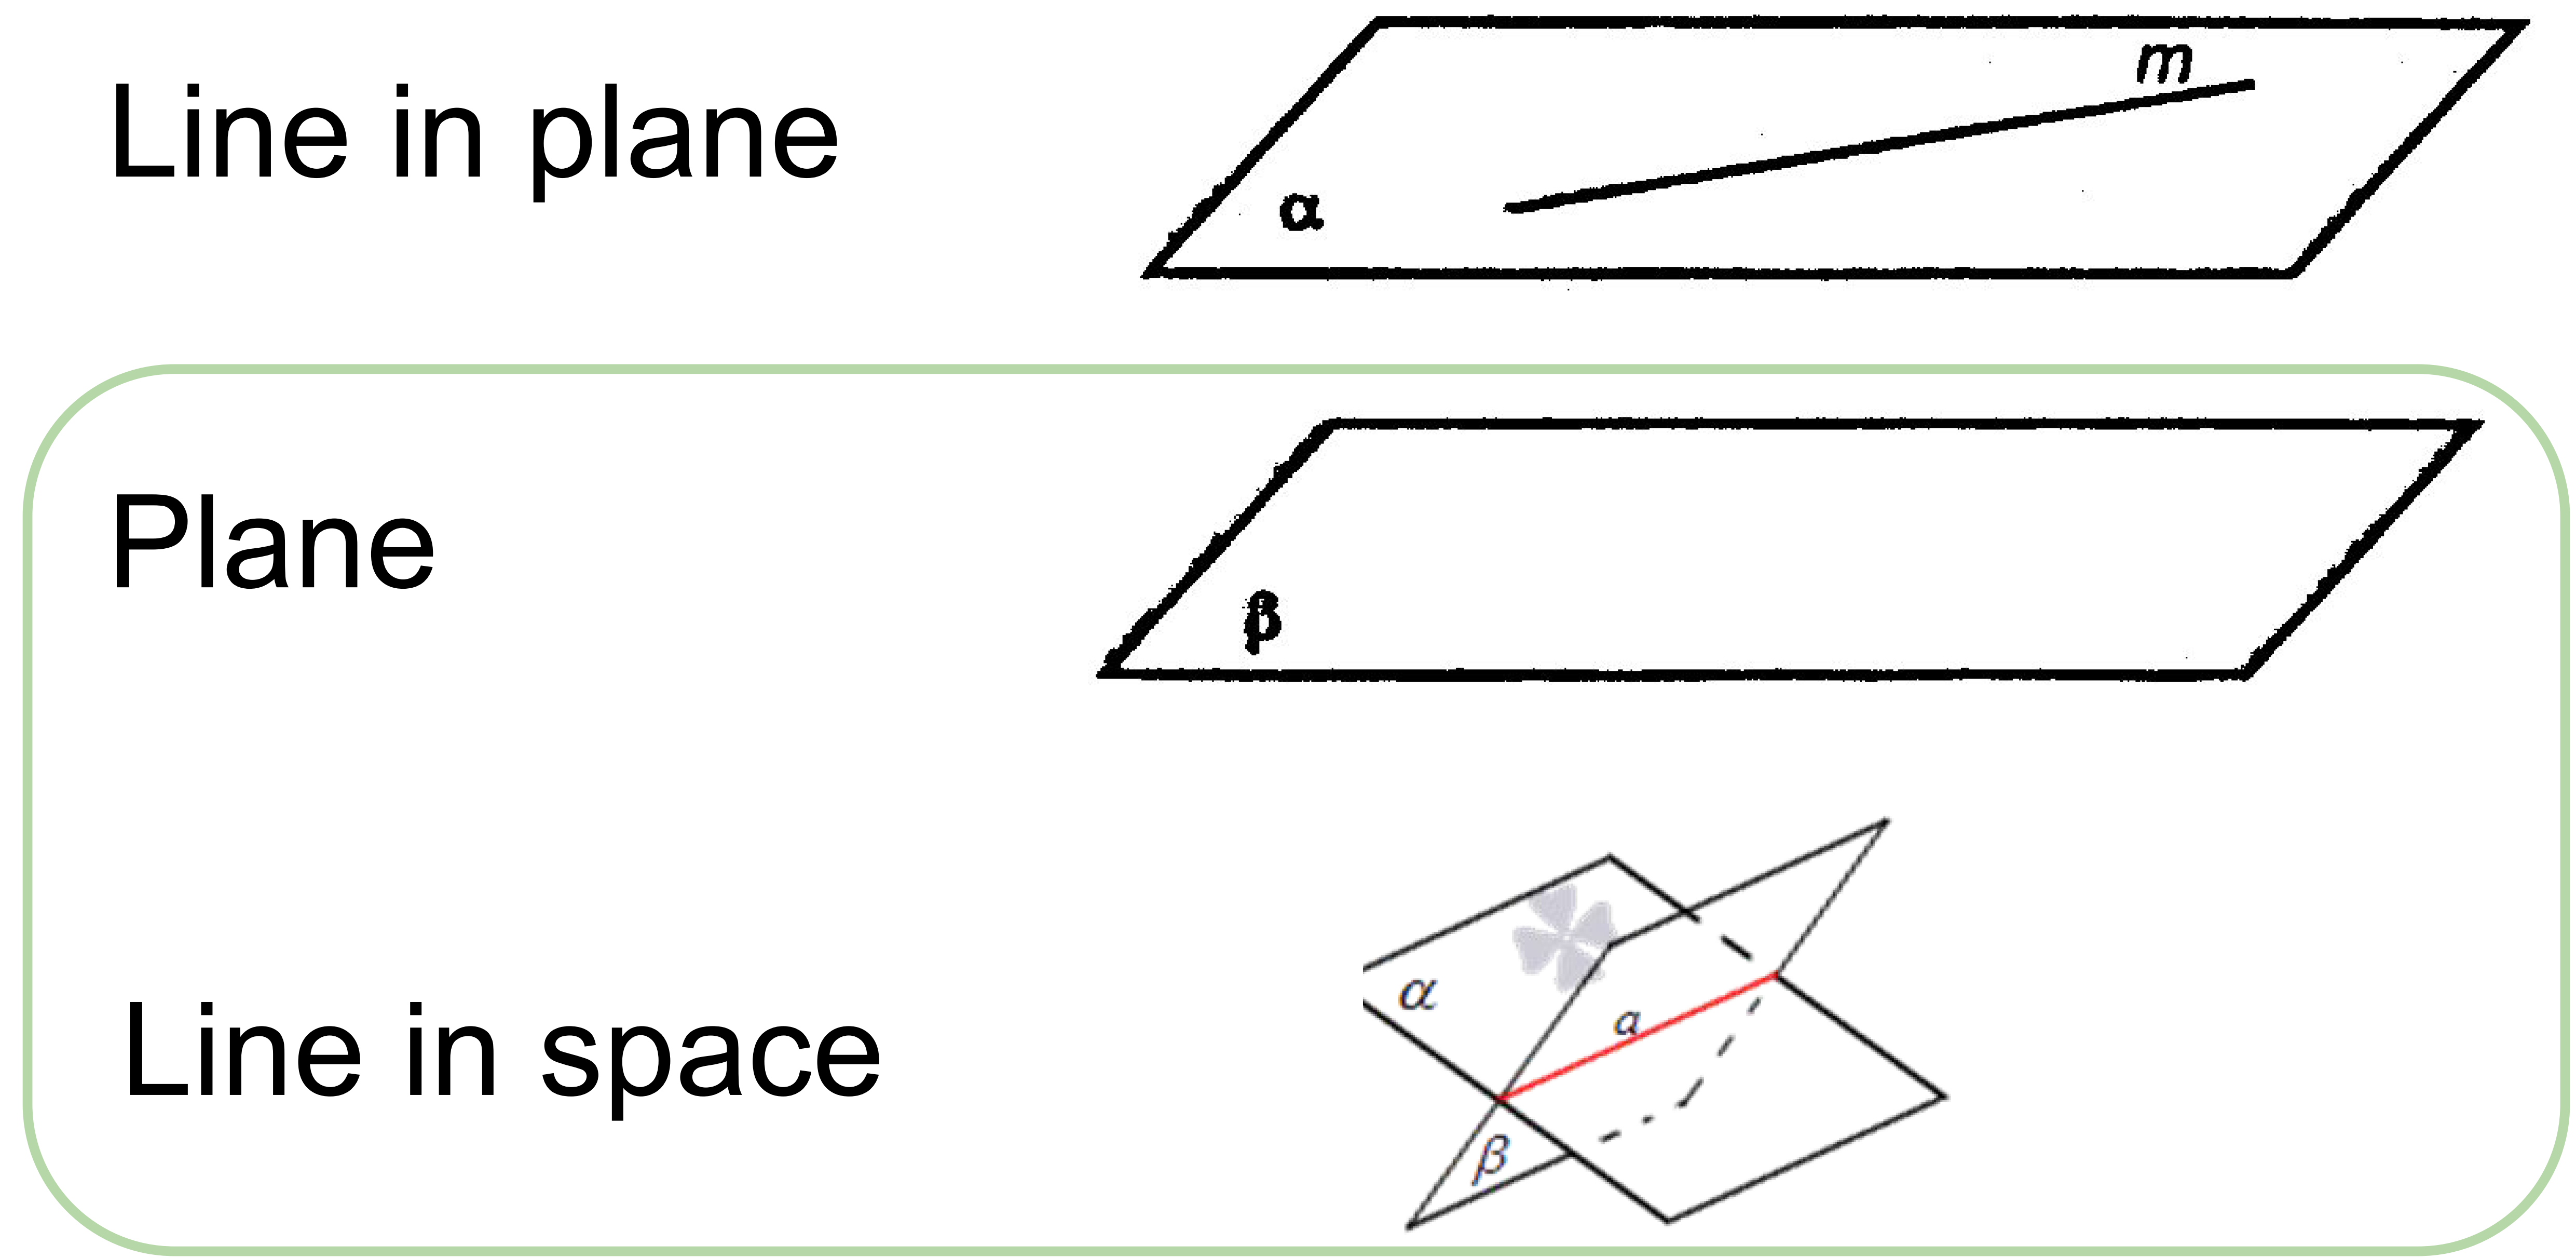
\includegraphics[height=6cm,width=1\textwidth,keepaspectratio]{plane_line_in_space.png}
        \label{fig:plane_line_in_space.png}
    \end{figure}
\end{frame}

\begin{frame}[t]{Plane}
    \framesubtitle{Formulas}
    \scriptsize
    \vspace{-0.4cm}
    \begin{multicols}{2}
        \begin{enumerate}
            \item \textbf{\textit{General}} $Ax + By + Cz + D = 0$, where \\ $D = -Ax_0 - By_0 - Cz_0$
            \item \textbf{\textit{Point-normal}} $(\vec{r} - \vec{r_0}) \cdot \vec{n} = 0$, where $\vec{n} = \begin{bmatrix}A\\B\\C \end{bmatrix}$, $\vec{r} = \begin{bmatrix}x\\y\\z \end{bmatrix}$, $\vec{r_0} = \begin{bmatrix}x_0\\y_0\\z_0 \end{bmatrix}$
            \item \textbf{\textit{In segments}} $\dfrac{x}{a} + \dfrac{y}{b} + \dfrac{z}{c} = 1$,\\ where $a=-\frac{D}{A}$, $b=-\frac{D}{B}$, $c=-\frac{D}{C}$ are points of intersection with the corresponded axes
            \item \textbf{\textit{Through three points}} $\begin{vmatrix}
                          x-x_1   & y-y_1   & z-z_1   \\
                          x_2-x_1 & y_2-y_1 & z_2-z_1 \\
                          x_3-x_1 & y_3-y_1 & z_3-z_1
                      \end{vmatrix} = 0 $, where \\ $x_{1,2,3}$, $y_{1,2,3}$, $z_{1,2,3}$ are some particular coordinates of points on the plane
            \item \textbf{\textit{Parametric}} $\vec{r} = \vec{r_0} + \alpha \vec{u} + \beta \vec{v} = \left\{\begin{matrix} x = x_0 + \alpha u_x + \beta v_x
                          \\ y = y_0 + \alpha u_y + \beta v_y \\ z = z_0 + \alpha u_z + \beta v_z
                      \end{matrix}\right. $, \\where $\vec{r_0}$ -- some point on a plane,\\ $\vec{u}$, $\vec{v}$ -- direction vectors, $\alpha$, $\beta$ are parameters
        \end{enumerate}
    \end{multicols}
\end{frame}

\begin{frame}[t]{Plane}
    \framesubtitle{Task 0}
    \begin{minipage}{0.49\textwidth}
        \begin{enumerate}
            \item Write down all forms of the line
            \item Draw this plane
        \end{enumerate}

    \end{minipage}
    \begin{minipage}{0.5\textwidth}
        \begin{align*}
            \frac{x}{2}+\frac{y}{1}+\frac{z}{3}=1
        \end{align*}
    \end{minipage}
\end{frame}

\begin{frame}[t]{Plane}
    \framesubtitle{Task 0, Answer}
    \vspace{-0.6cm}
    \begin{figure}[H]
        \href{https://www.geogebra.org/m/rxduxkwn}{
            \centering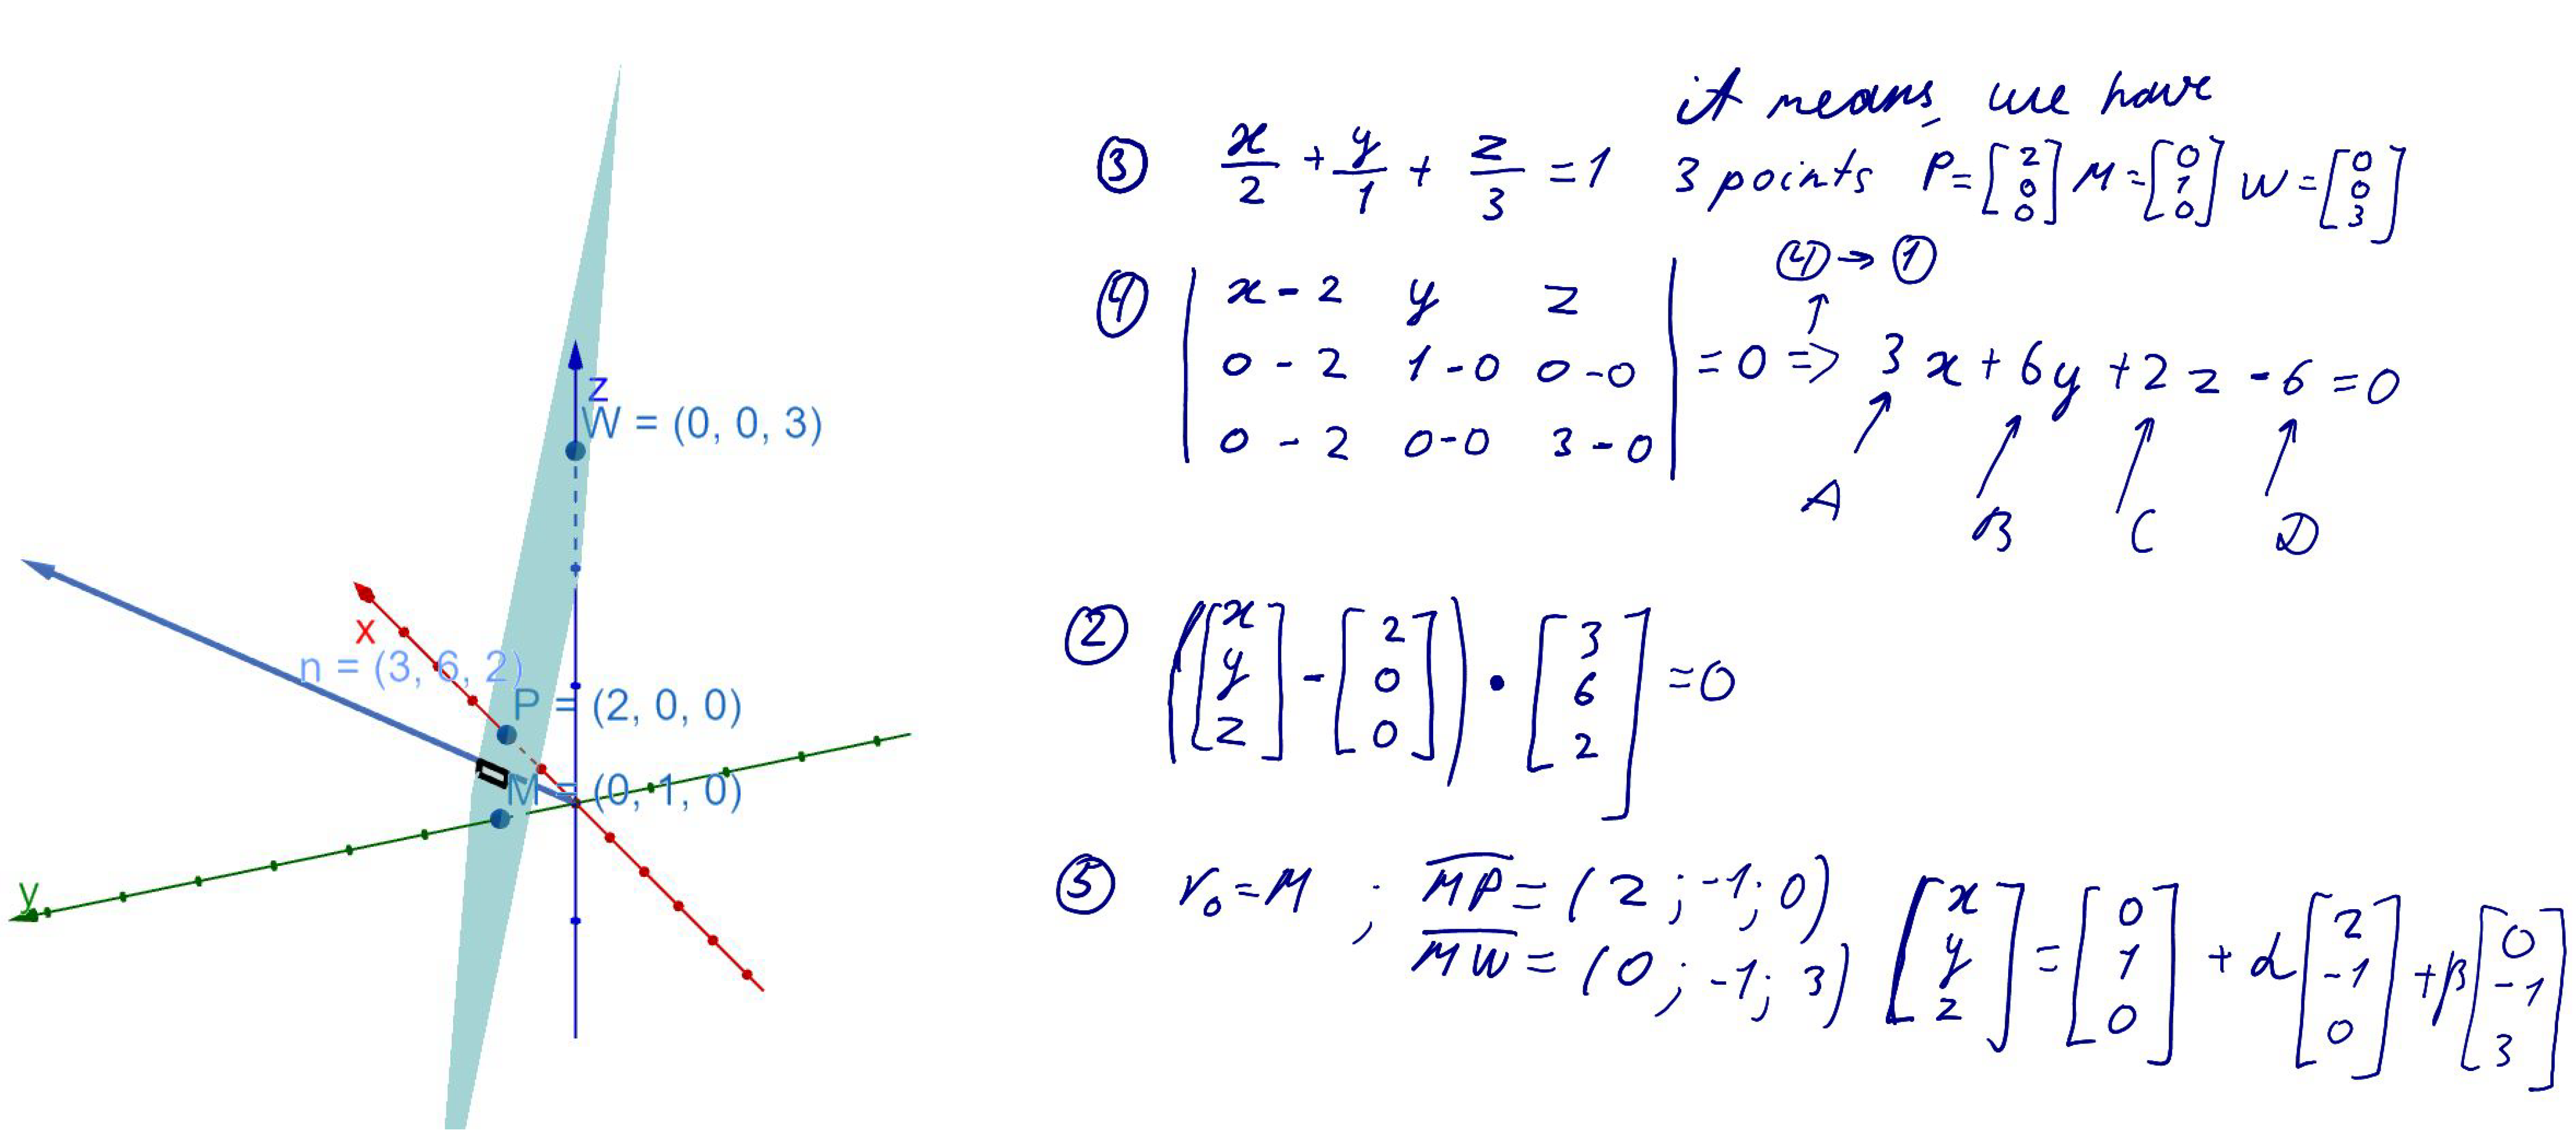
\includegraphics[height=6cm,width=1\textwidth,keepaspectratio]{plane_ans.png}}
        % \caption{Click on a picture for a video}
        \label{fig:plane_ans.png}
    \end{figure}
\end{frame}

\begin{frame}[t]{Task 1}
    \framesubtitle{}
    \only<1>{
        Find the equation of the plane passing through the point $(2, -3, 4)$ and parallel to the plane $2x - 5y - 7z + 15 = 0$. And draw the picture.}
    \only<2>{
        \alert{\Large Answer}
        \begin{figure}[H]
            \centering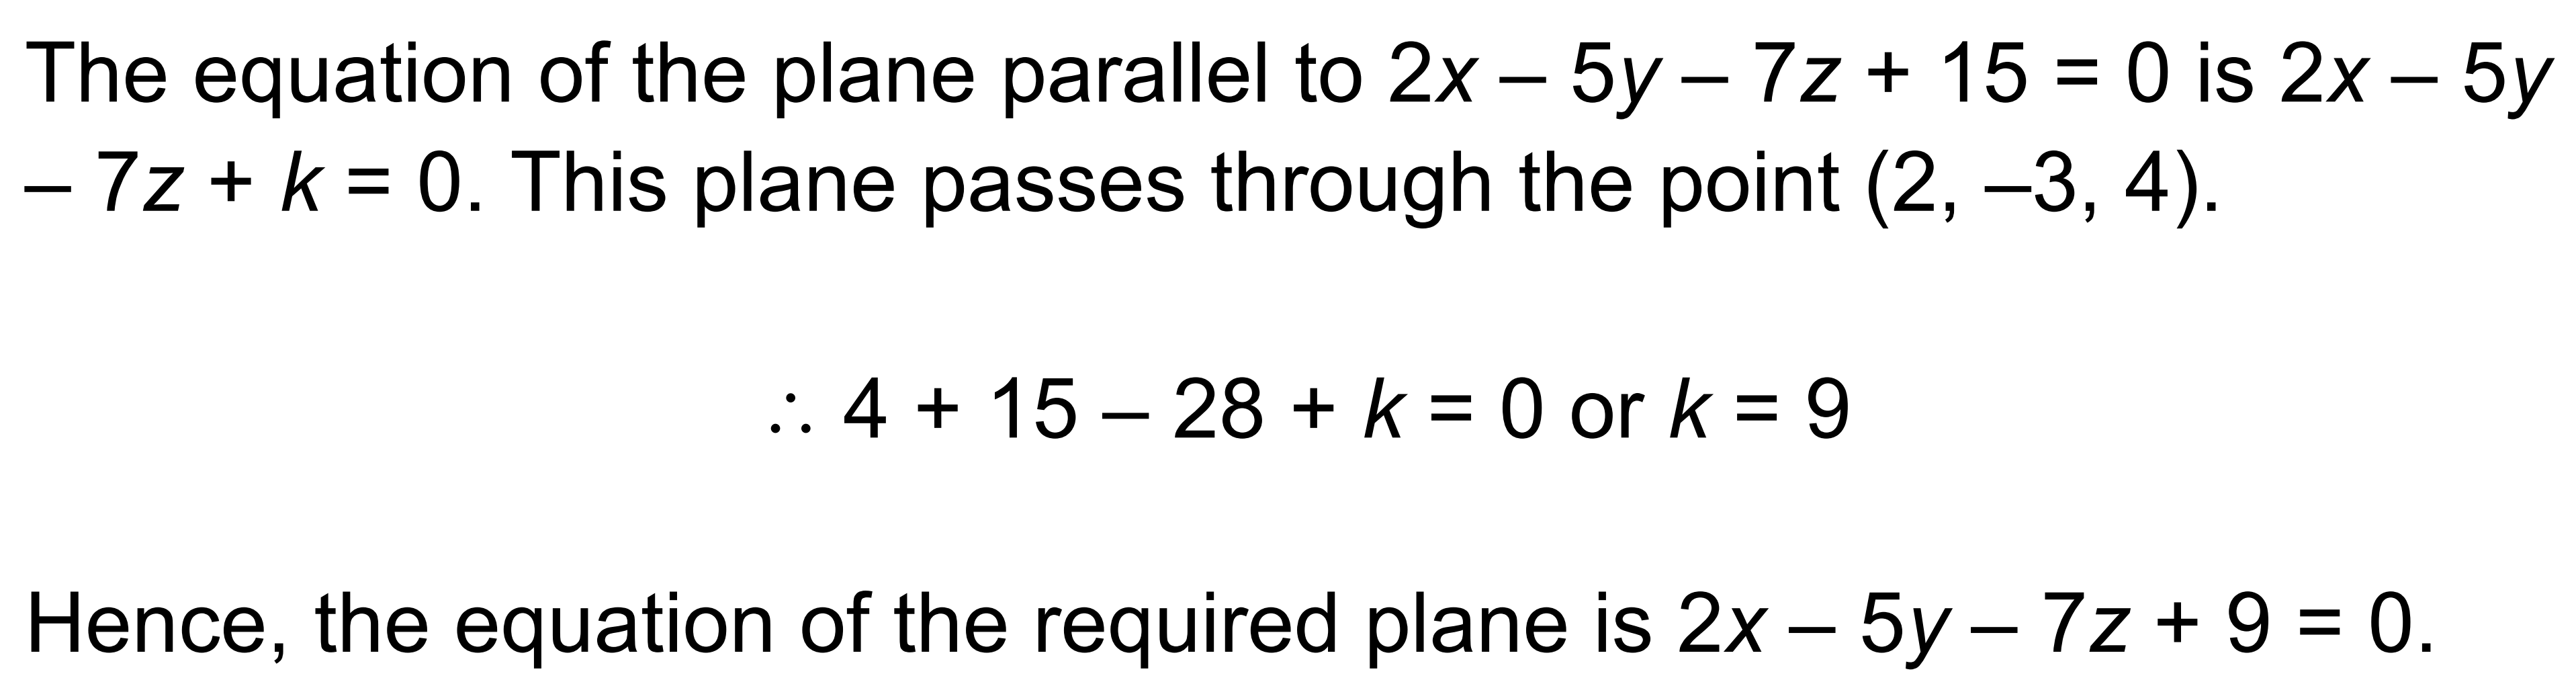
\includegraphics[height=5.5cm,width=1\textwidth,keepaspectratio]{1ans.png}
            % \caption{caption_name}
            \label{fig:1ans.png}
        \end{figure}
    }
\end{frame}

\begin{frame}[t]{Line in space}
    \framesubtitle{Formulas}
    \scriptsize
    \vspace{-0.4cm}
    \begin{multicols}{2}
        \begin{enumerate}
            \item \textbf{\textit{Passing through two points}} $\dfrac{x-x_1}{x_2-x_1} = \dfrac{y-y_1}{y_2-y_1}=\dfrac{z-z_1}{z_2-z_1}$\\ where $x_{1,2}$, $y_{1,2}$, $z_{1,2}$ are some particular coordinates of points on the line
            \item \textbf{\textit{Canonical}} $\dfrac{x-x_0}{a_x} = \dfrac{y-y_0}{a_y}=\dfrac{z-z_0}{a_z}$,\\ where $x_0$, $y_0$, $z_0$ is a point on the line and $a_x$, $a_y$, $a_z$ -- direction vector coefficients on a basis
            \item \textbf{\textit{Parametric}} $\vec{r} = \vec{r_0} + \tau \vec{a}=\left\{\begin{matrix} x = x_0 + \tau a_x
                          \\ y = y_0 + \tau a_y \\ z = z_0 + \tau a_z
                      \end{matrix}\right.$, where $\tau$ is parameter,\\ which can be received from canonical form ($\dfrac{x-x_0}{a_x} = \dfrac{y-y_0}{a_y} =\dfrac{z-z_0}{a_z}= \tau$)
            \item \textbf{\textit{General}} $\left\{\begin{matrix} A_1x + B_1y + C_1z + D_1 = 0
                          \\ A_2x + B_2y + C_2z + D_2 = 0
                      \end{matrix}\right.$, where \\ $D_{1,2} = -A_{1,2}x_0 - B_{1,2}y_0 - C_{1,2}z_0$
            \item \textbf{\textit{Point - 2 normal lines}} $\left\{\begin{matrix}(\vec{r} - \vec{r_0}) \cdot \vec{n_1} = 0 \\ (\vec{r} - \vec{r_0}) \cdot \vec{n_2} = 0 \end{matrix}\right.$, where $\vec{n} = \begin{bmatrix}A\\B\\C \end{bmatrix}$, $\vec{r} = \begin{bmatrix}x\\y\\z \end{bmatrix}$, $\vec{r_0} = \begin{bmatrix}x_0\\y_0\\z_0 \end{bmatrix}$
            \item \textbf{\textit{Point - direction vector}} $\vec{a} \times (\vec{r}-\vec{r_0}) = 0$, where $\vec{a} = \vec{n_1}\times\vec{n_2}$
            \item[\vspace{\fill}]
            \item[\vspace{\fill}]
        \end{enumerate}
    \end{multicols}
\end{frame}

\begin{frame}[t]{Line in space}
    \framesubtitle{Task 0}
    \begin{minipage}{0.49\textwidth}
        \begin{enumerate}
            \item Write down all forms of the line
            \item Draw this line
        \end{enumerate}

    \end{minipage}
    \begin{minipage}{0.5\textwidth}
        \begin{align*}
            \left\{\begin{matrix*}[l]
                       15x+9y+0z-45=0\\
                       0x-8y+0z=0
                   \end{matrix*}\right.
        \end{align*}
    \end{minipage}
\end{frame}

\begin{frame}[t]{Line in space}
    \framesubtitle{Task 0, Answer}
    \vspace{-0.6cm}
    \begin{figure}[H]
        \href{https://www.geogebra.org/3d/mfyfgc9z}{
            \centering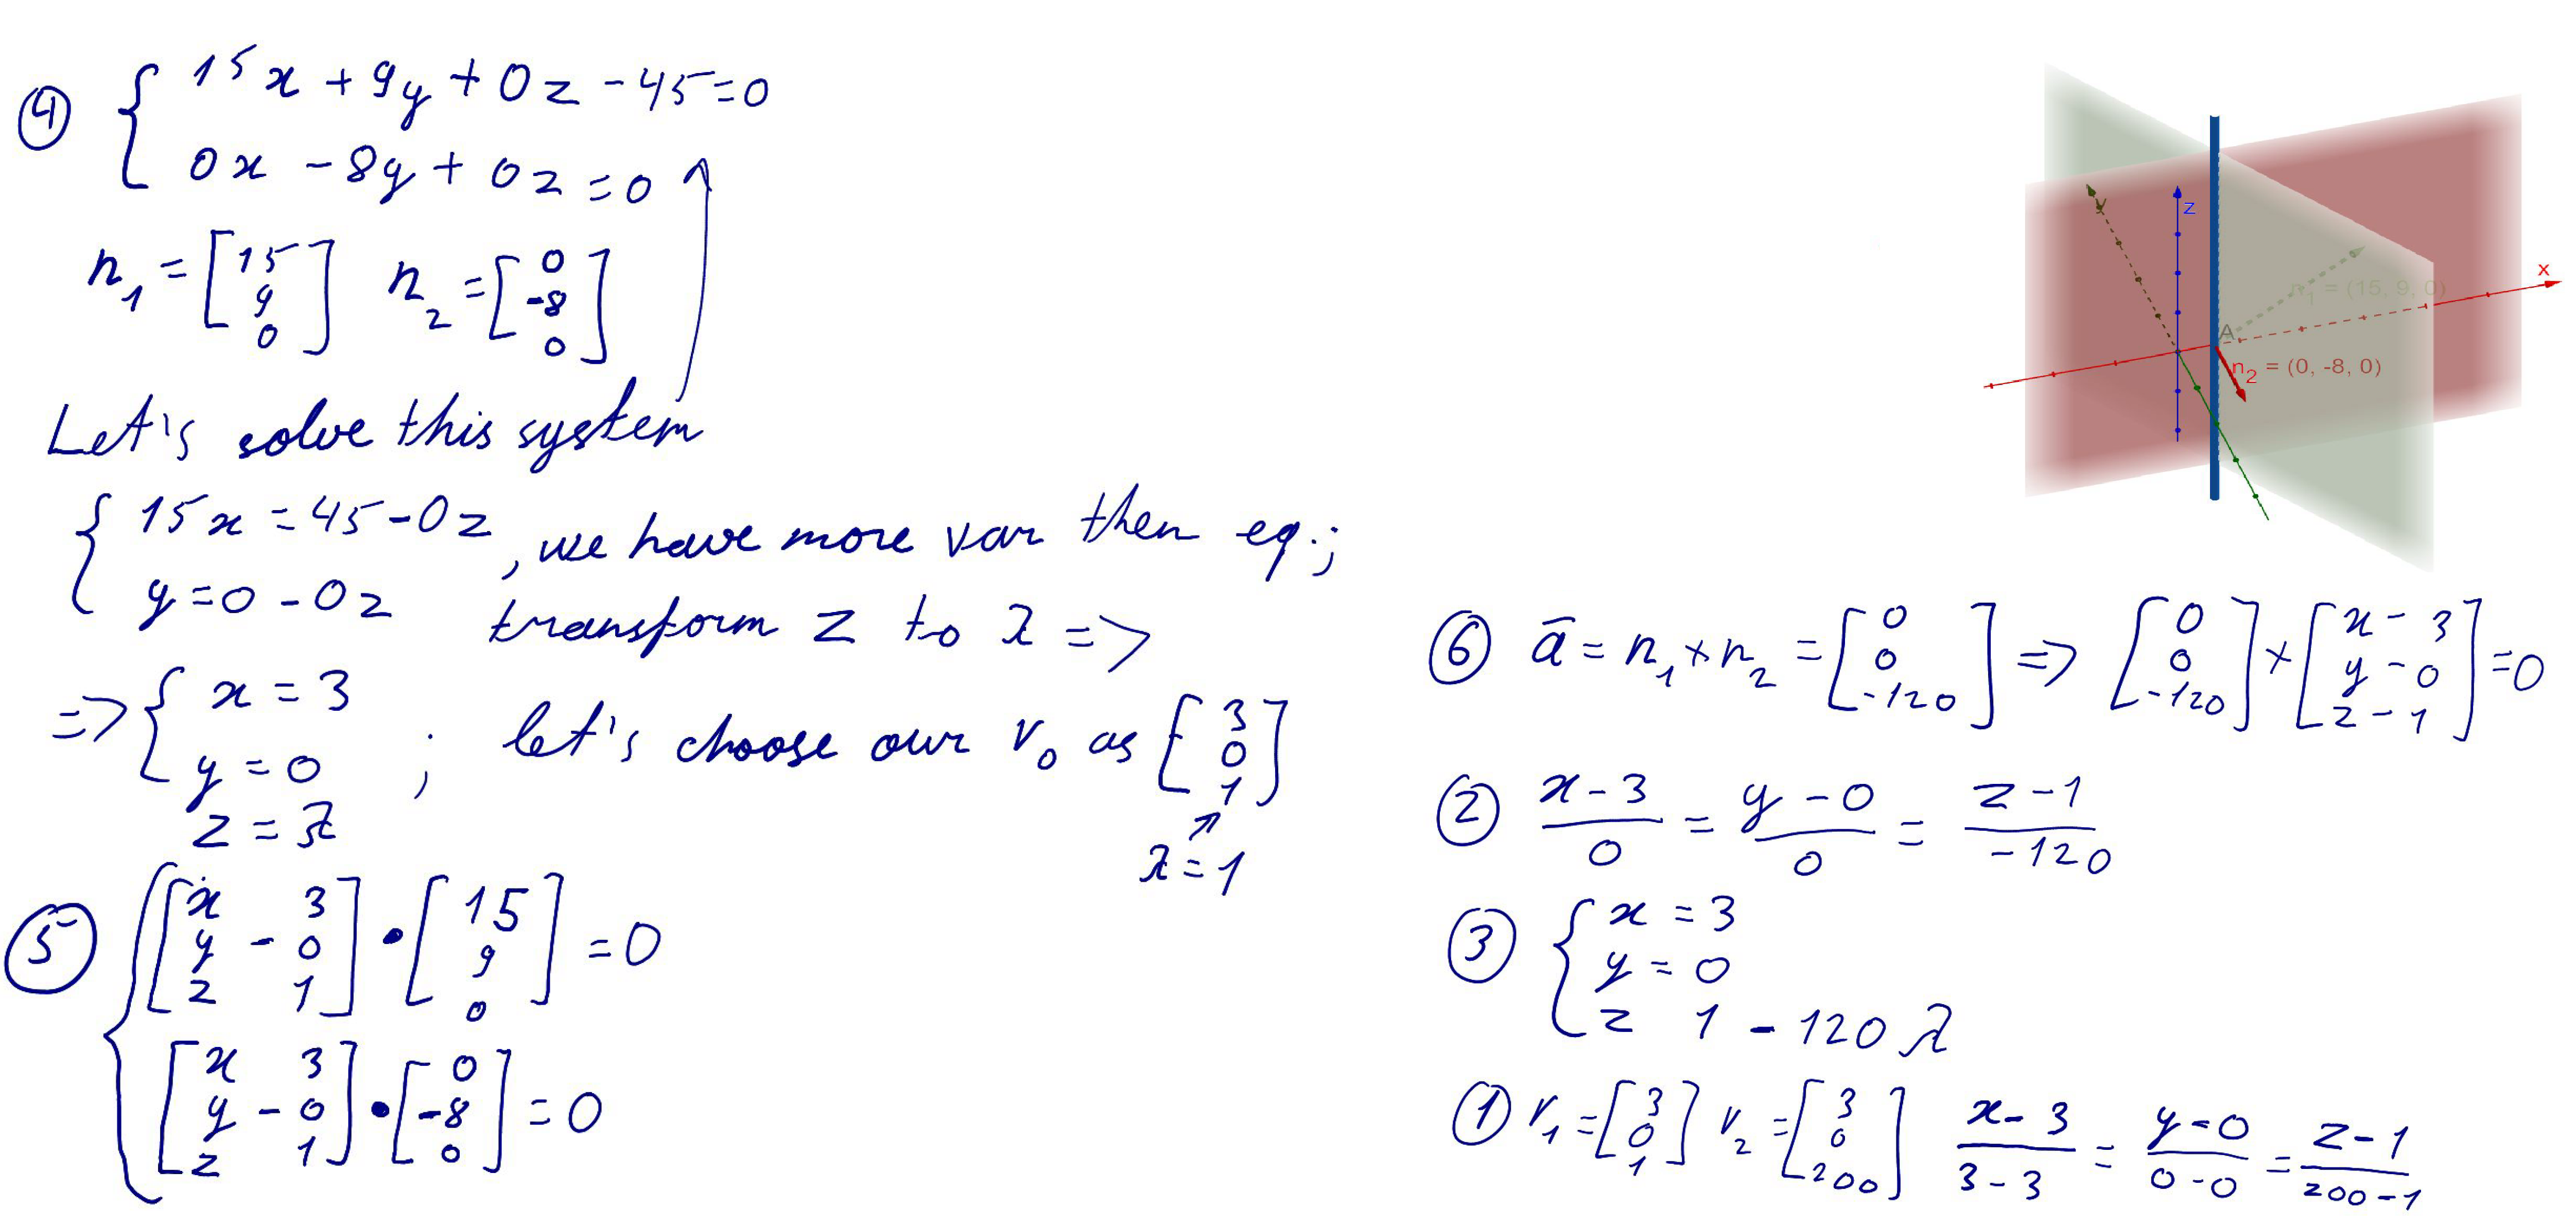
\includegraphics[height=6cm,width=1\textwidth,keepaspectratio]{line_in_space_ans.png}}
        % \caption{Click on a picture for a video}
        \label{fig:line_in_space_ans.png}
    \end{figure}
\end{frame}

\begin{frame}[t]{Task 2}
    \framesubtitle{}
    \only<1>{
        \begin{minipage}{0.6\textwidth}
            Find the equations of the line passing through the point $(1, 2, 3)$ and \underline{perpendicular to the planes} $x - 2y - z + 5 = 0$ and $x + y + 3z + 6 = 0$. And draw the picture. \medskip

            \alert{\underline{perpendicular to the planes}} --- it cannot be physically (typo). It should be either "Perpendicualr to the normals of planes", or "parallel to the planes".
        \end{minipage}
        \begin{minipage}{0.39\textwidth}
            \begin{figure}[H]
                \href{https://www.geogebra.org/3d/ypbugjzu}{
                    \centering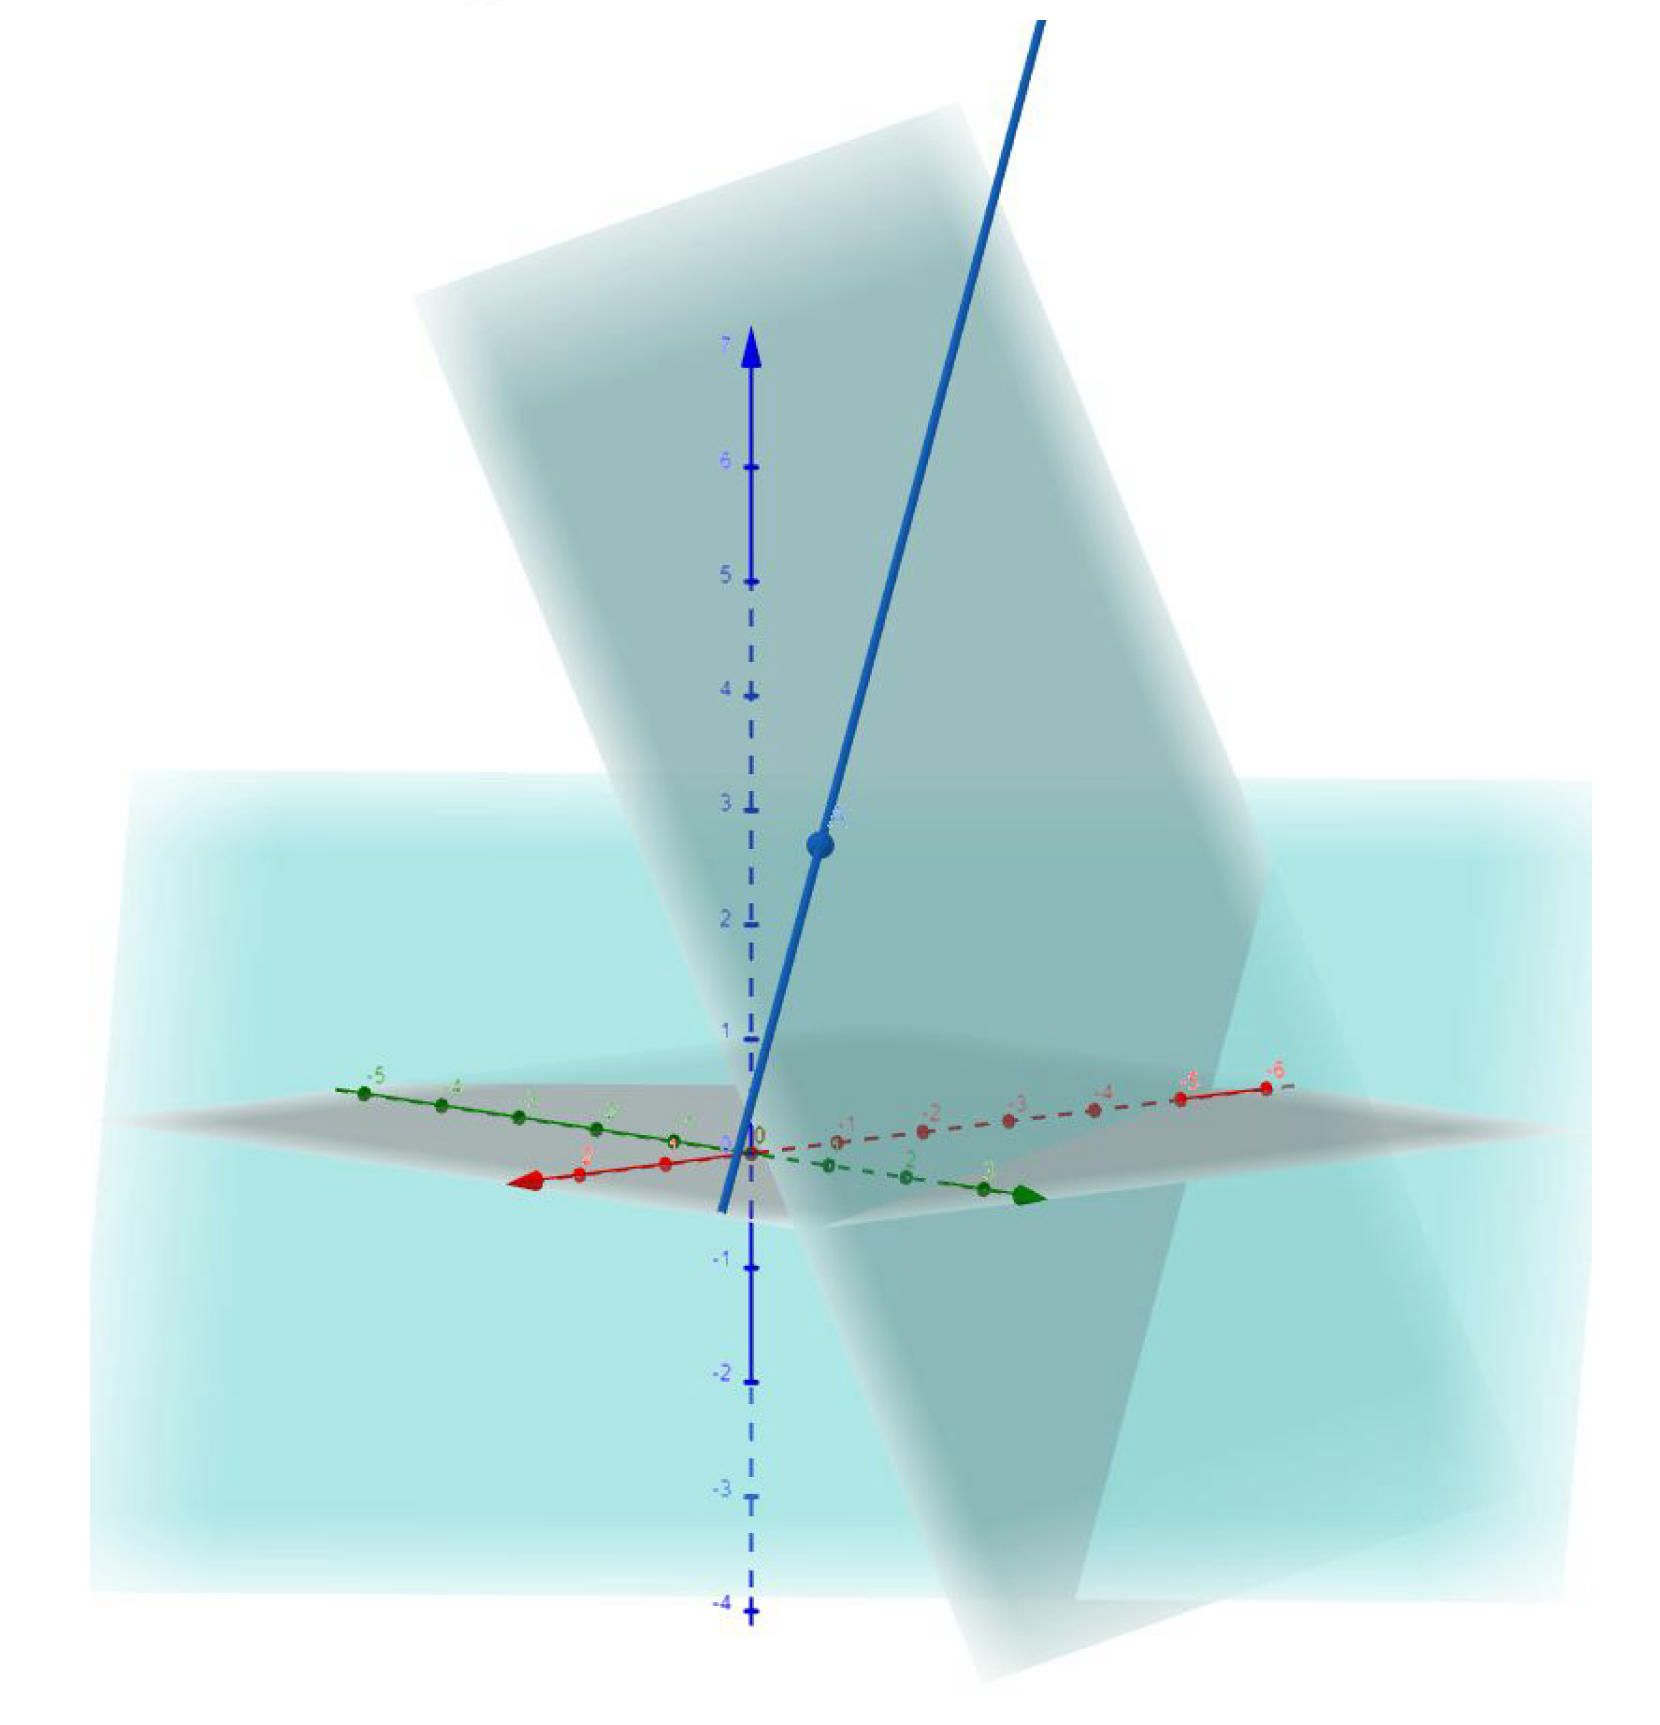
\includegraphics[height=6cm,width=1\textwidth,keepaspectratio]{2_fig.png}}
                % \caption{caption_name}
                \label{fig:2_fig.png}
            \end{figure}
        \end{minipage}}
    \only<2>{
        \alert{\Large Answer}
        \begin{figure}[H]
            \centering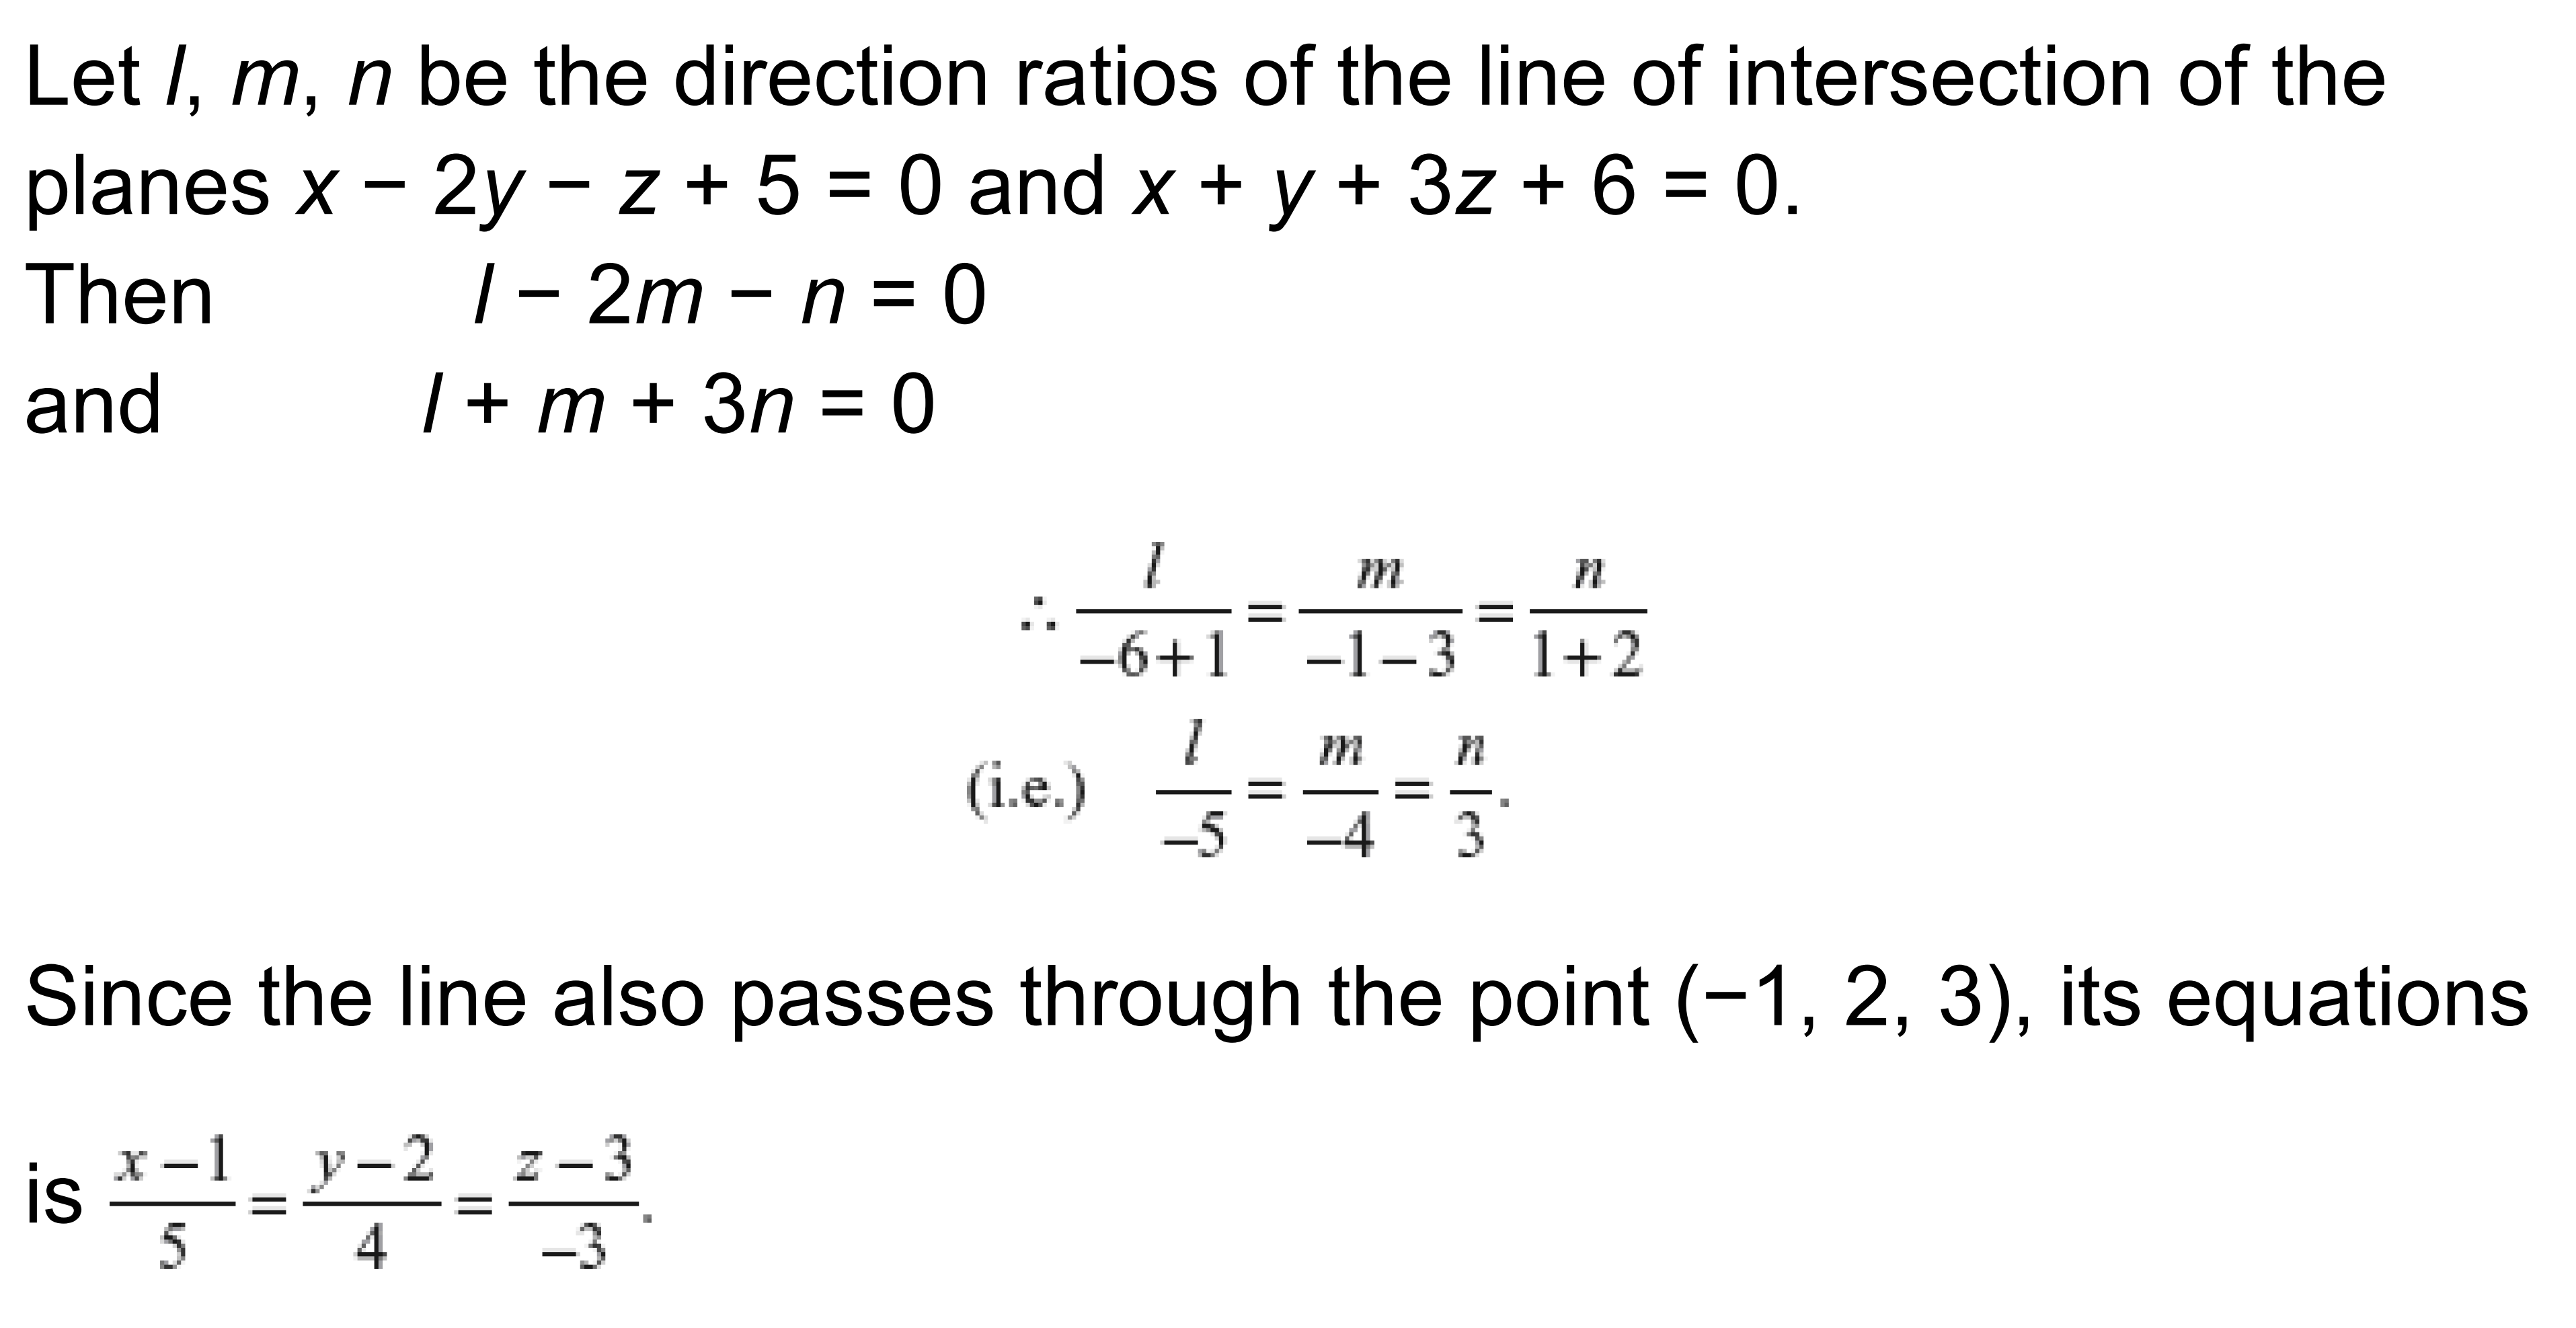
\includegraphics[height=5.5cm,width=1\textwidth,keepaspectratio]{2ans.png}
            % \caption{caption_name}
            \label{fig:2ans.png}
        \end{figure}
    }
\end{frame}

\begin{frame}[t]{Task 3}
    \framesubtitle{}
    \only<1>{
        \begin{minipage}{0.6\textwidth}
            Find the equation of the plane which passes through the intersection of the planes $2x + 3y + 10z - 8 = 0, 2x - 3y + 7z - 2 = 0$ and is perpendicular to the plane $3x - 2y + 4z - 5 = 0$. And draw the picture.
        \end{minipage}
        \begin{minipage}{0.39\textwidth}
            \begin{figure}[H]
                \href{https://www.geogebra.org/3d/ynkngnsv}{
                    \centering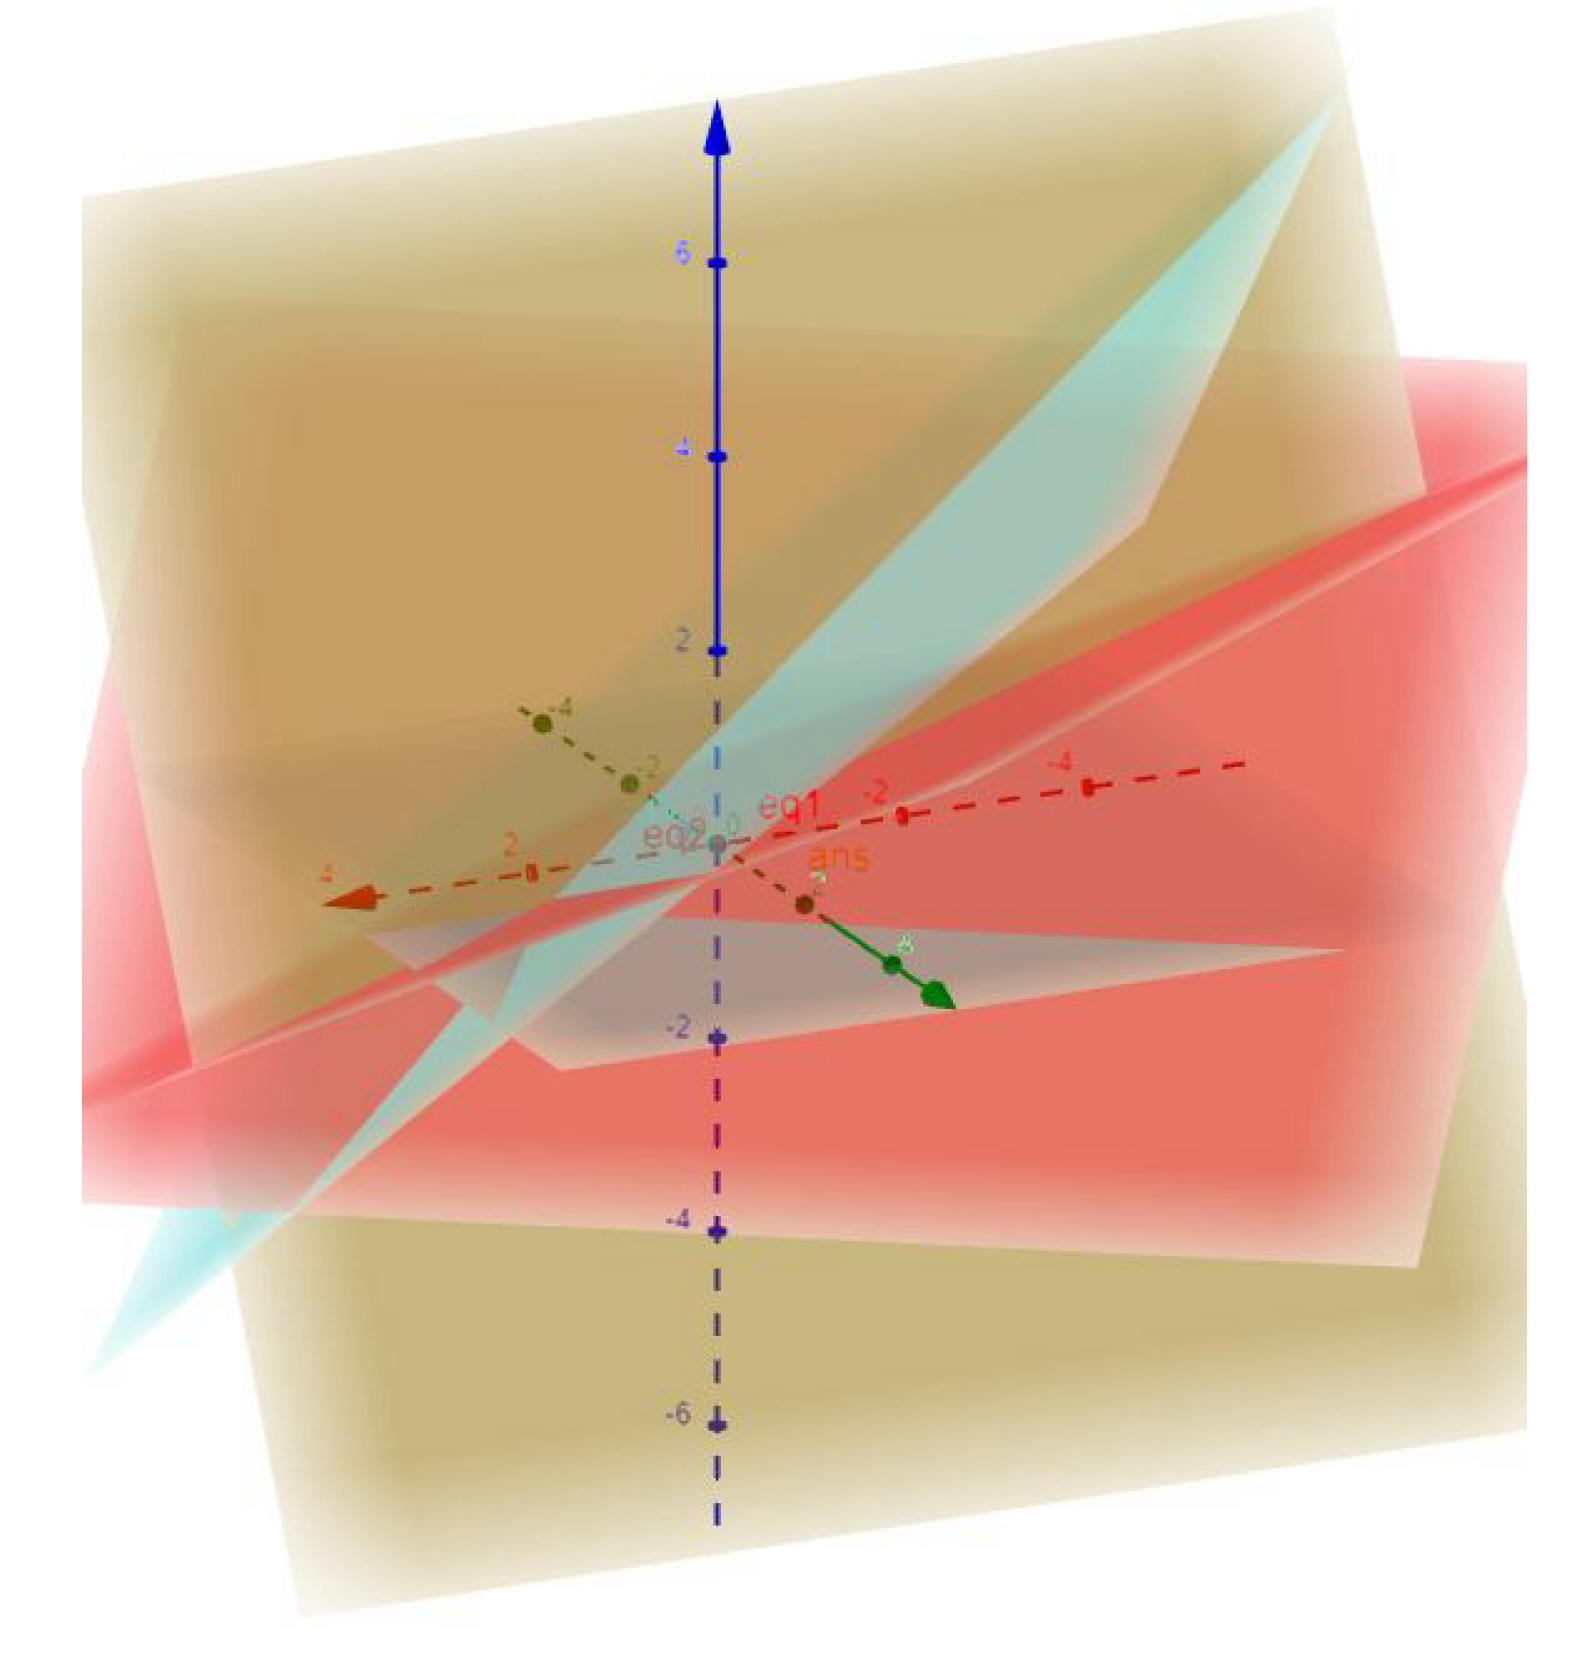
\includegraphics[height=6cm,width=1\textwidth,keepaspectratio]{3_fig.png}}
                % \caption{caption_name}
                \label{fig:3_fig.png}
            \end{figure}
        \end{minipage}}
    \only<2>{
        \alert{\Large Answer}
        \begin{figure}[H]
            \centering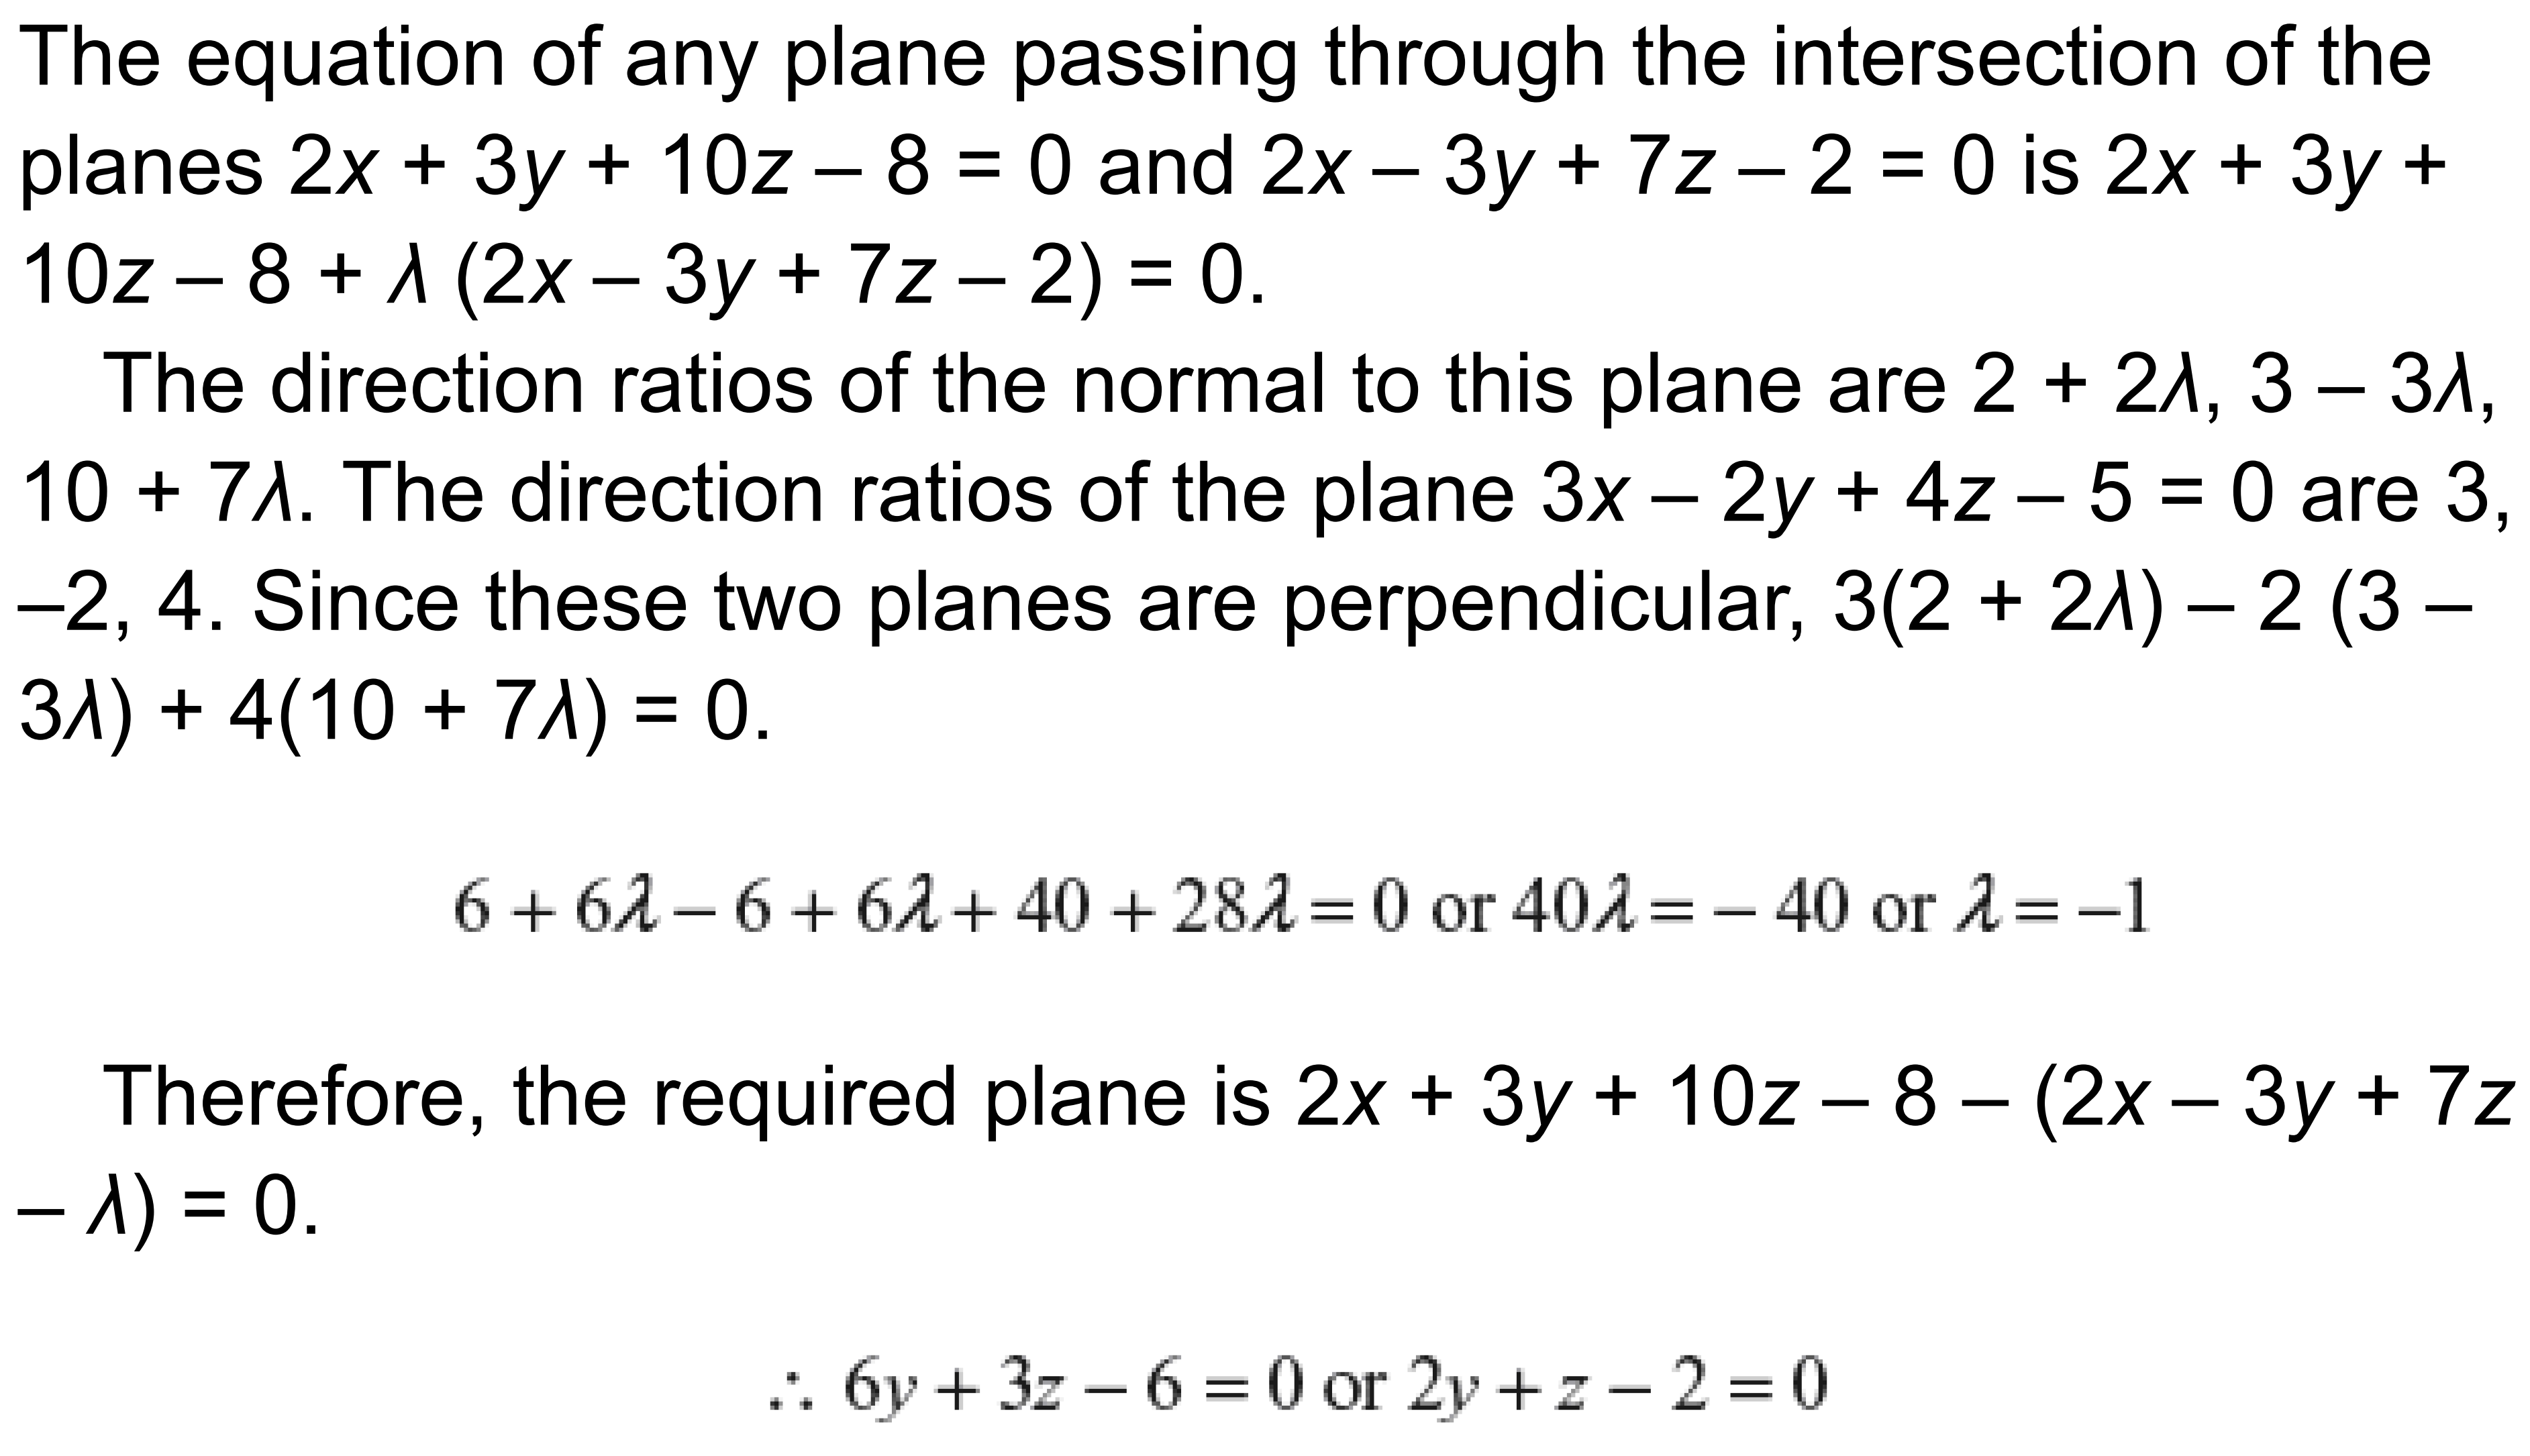
\includegraphics[height=5.5cm,width=1\textwidth,keepaspectratio]{3ans.png}
            % \caption{caption_name}
            \label{fig:3ans.png}
        \end{figure}
    }
\end{frame}

\begin{frame}[t]{}
    \begin{figure}[H]
        \href{http://www.youtube.com/watch?v=5-l-OkR5yDk}{
            \centering
\includegraphics[height=6cm,width=1\textwidth,keepaspectratio]{slav_adidas.jpg}}
        % \caption{Click on a picture for a video}
        \label{fig:slav_adidas.jpg}
    \end{figure}
\end{frame}

\begin{frame}[t]{Formulas of distances (Umnov 107)}
    \framesubtitle{Point to line}
    \begin{minipage}{0.6\textwidth}
        \textbf{\textit{Point to line}} $d = \dfrac{\left|(\vec{R}-\vec{r_0}) \times \vec{a}\right| }{\left|\vec{a}\right|}$, where \\ $\vec{R}$ - is a \textbf{point},\\ $a$ -- directed vector of a line, \\ $r_0$ -- point on this line
    \end{minipage}
    \begin{minipage}{0.39\textwidth}
        \begin{figure}[H]
            \centering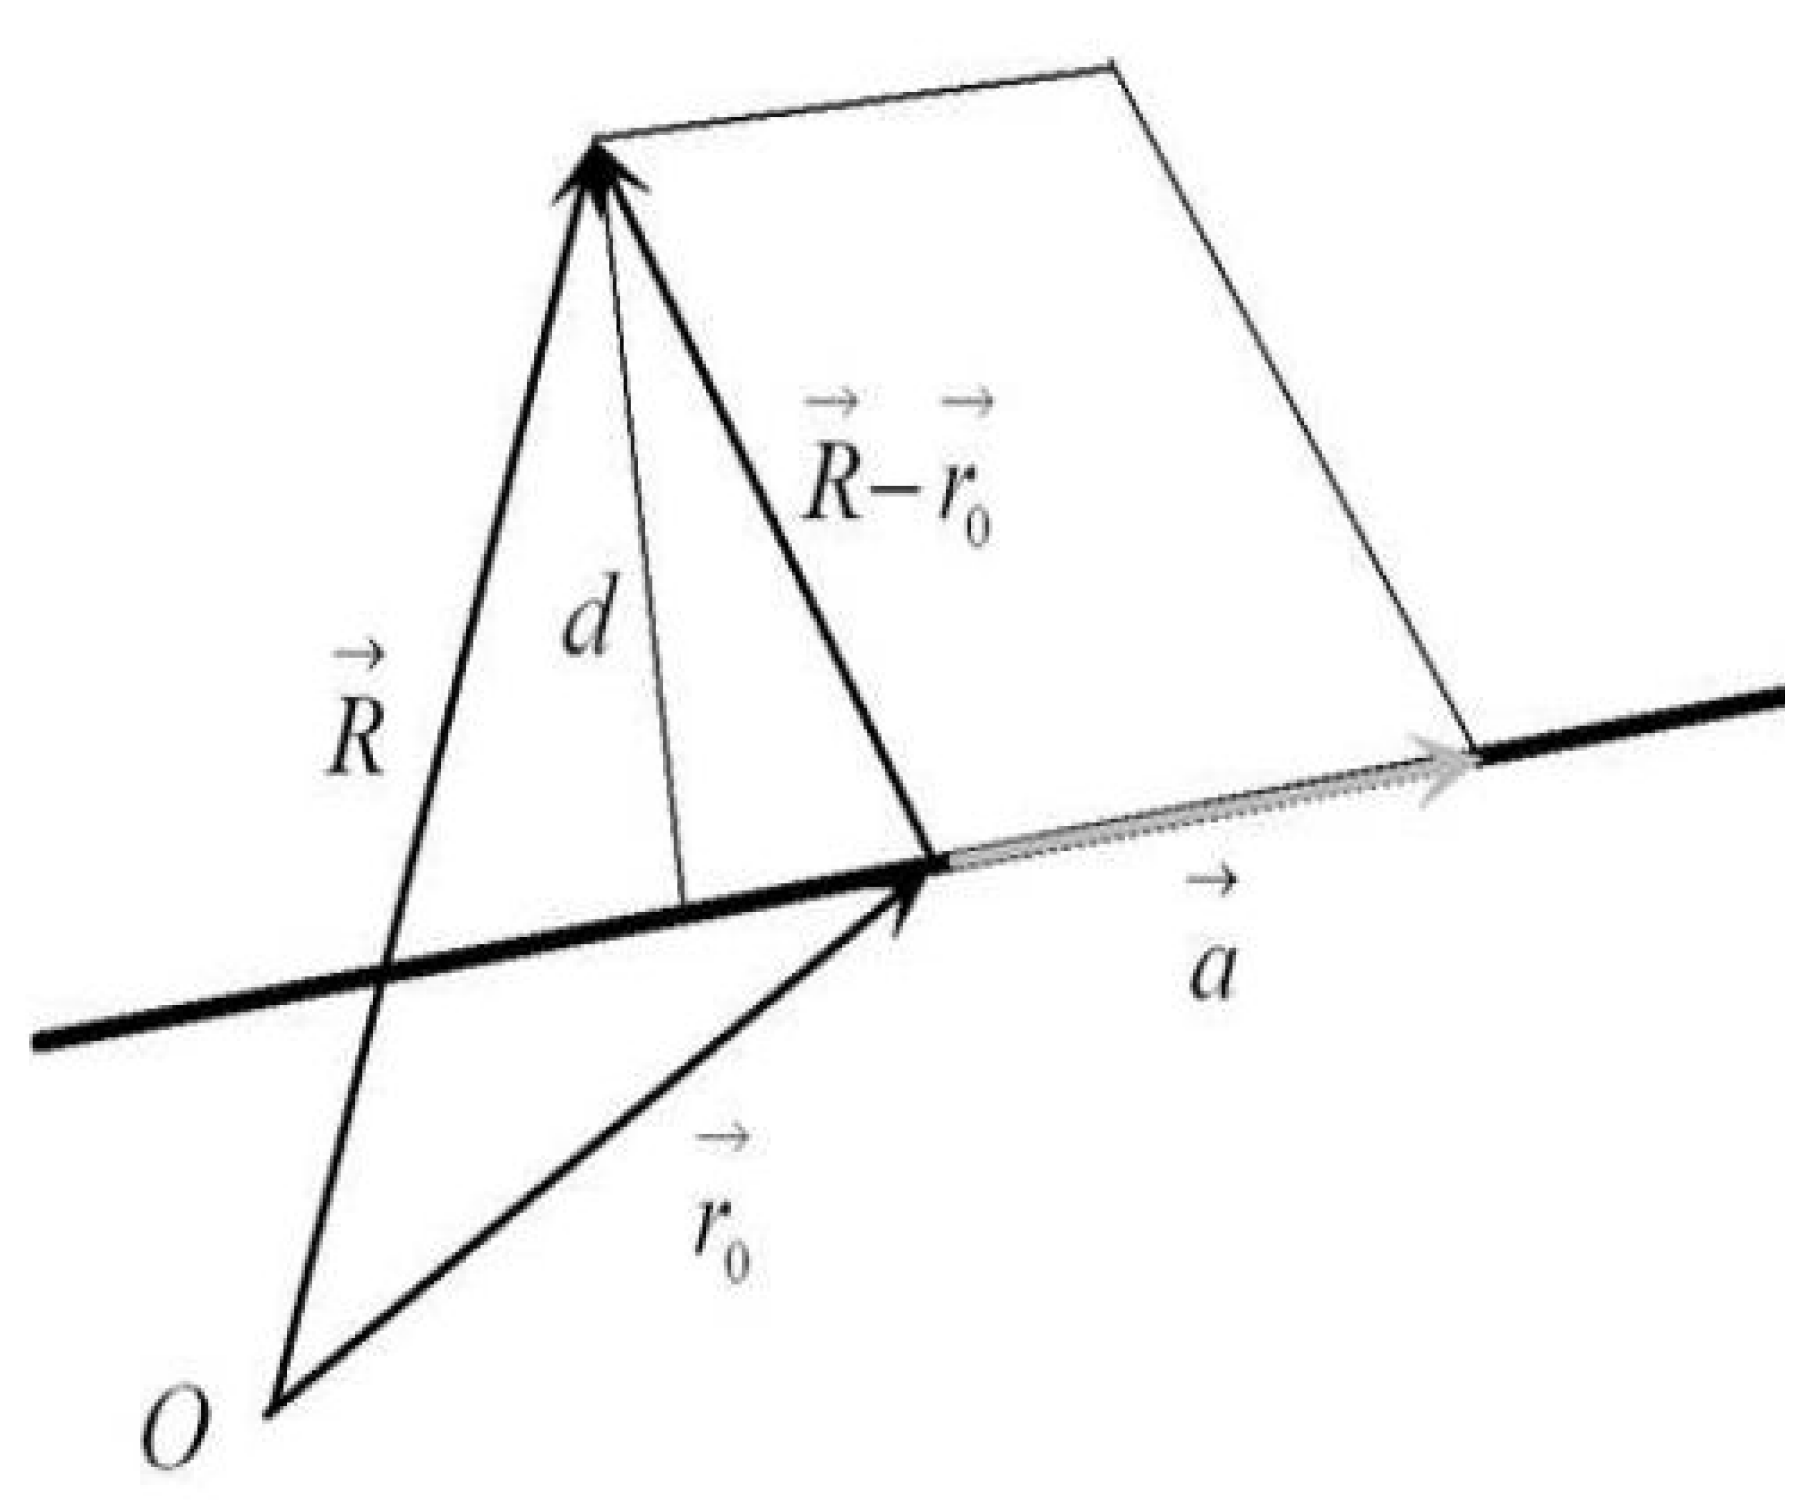
\includegraphics[height=4cm,width=1\textwidth,keepaspectratio]{distance_1.png}
            \label{fig:distance_1.png}
        \end{figure}
    \end{minipage}
\end{frame}

\begin{frame}[t]{Task 4}
    \framesubtitle{}
    \only<1>{
        Find the perpendicular distance from the point $(1, 3, -1)$ to the line \\ $\dfrac{x-13}{5} = \dfrac{y+8}{-8} = \dfrac{z-31}{1}$. And draw the picture.
    }
    \only<2>{
        \alert{\Large Answer}
        \begin{figure}[H]
            \centering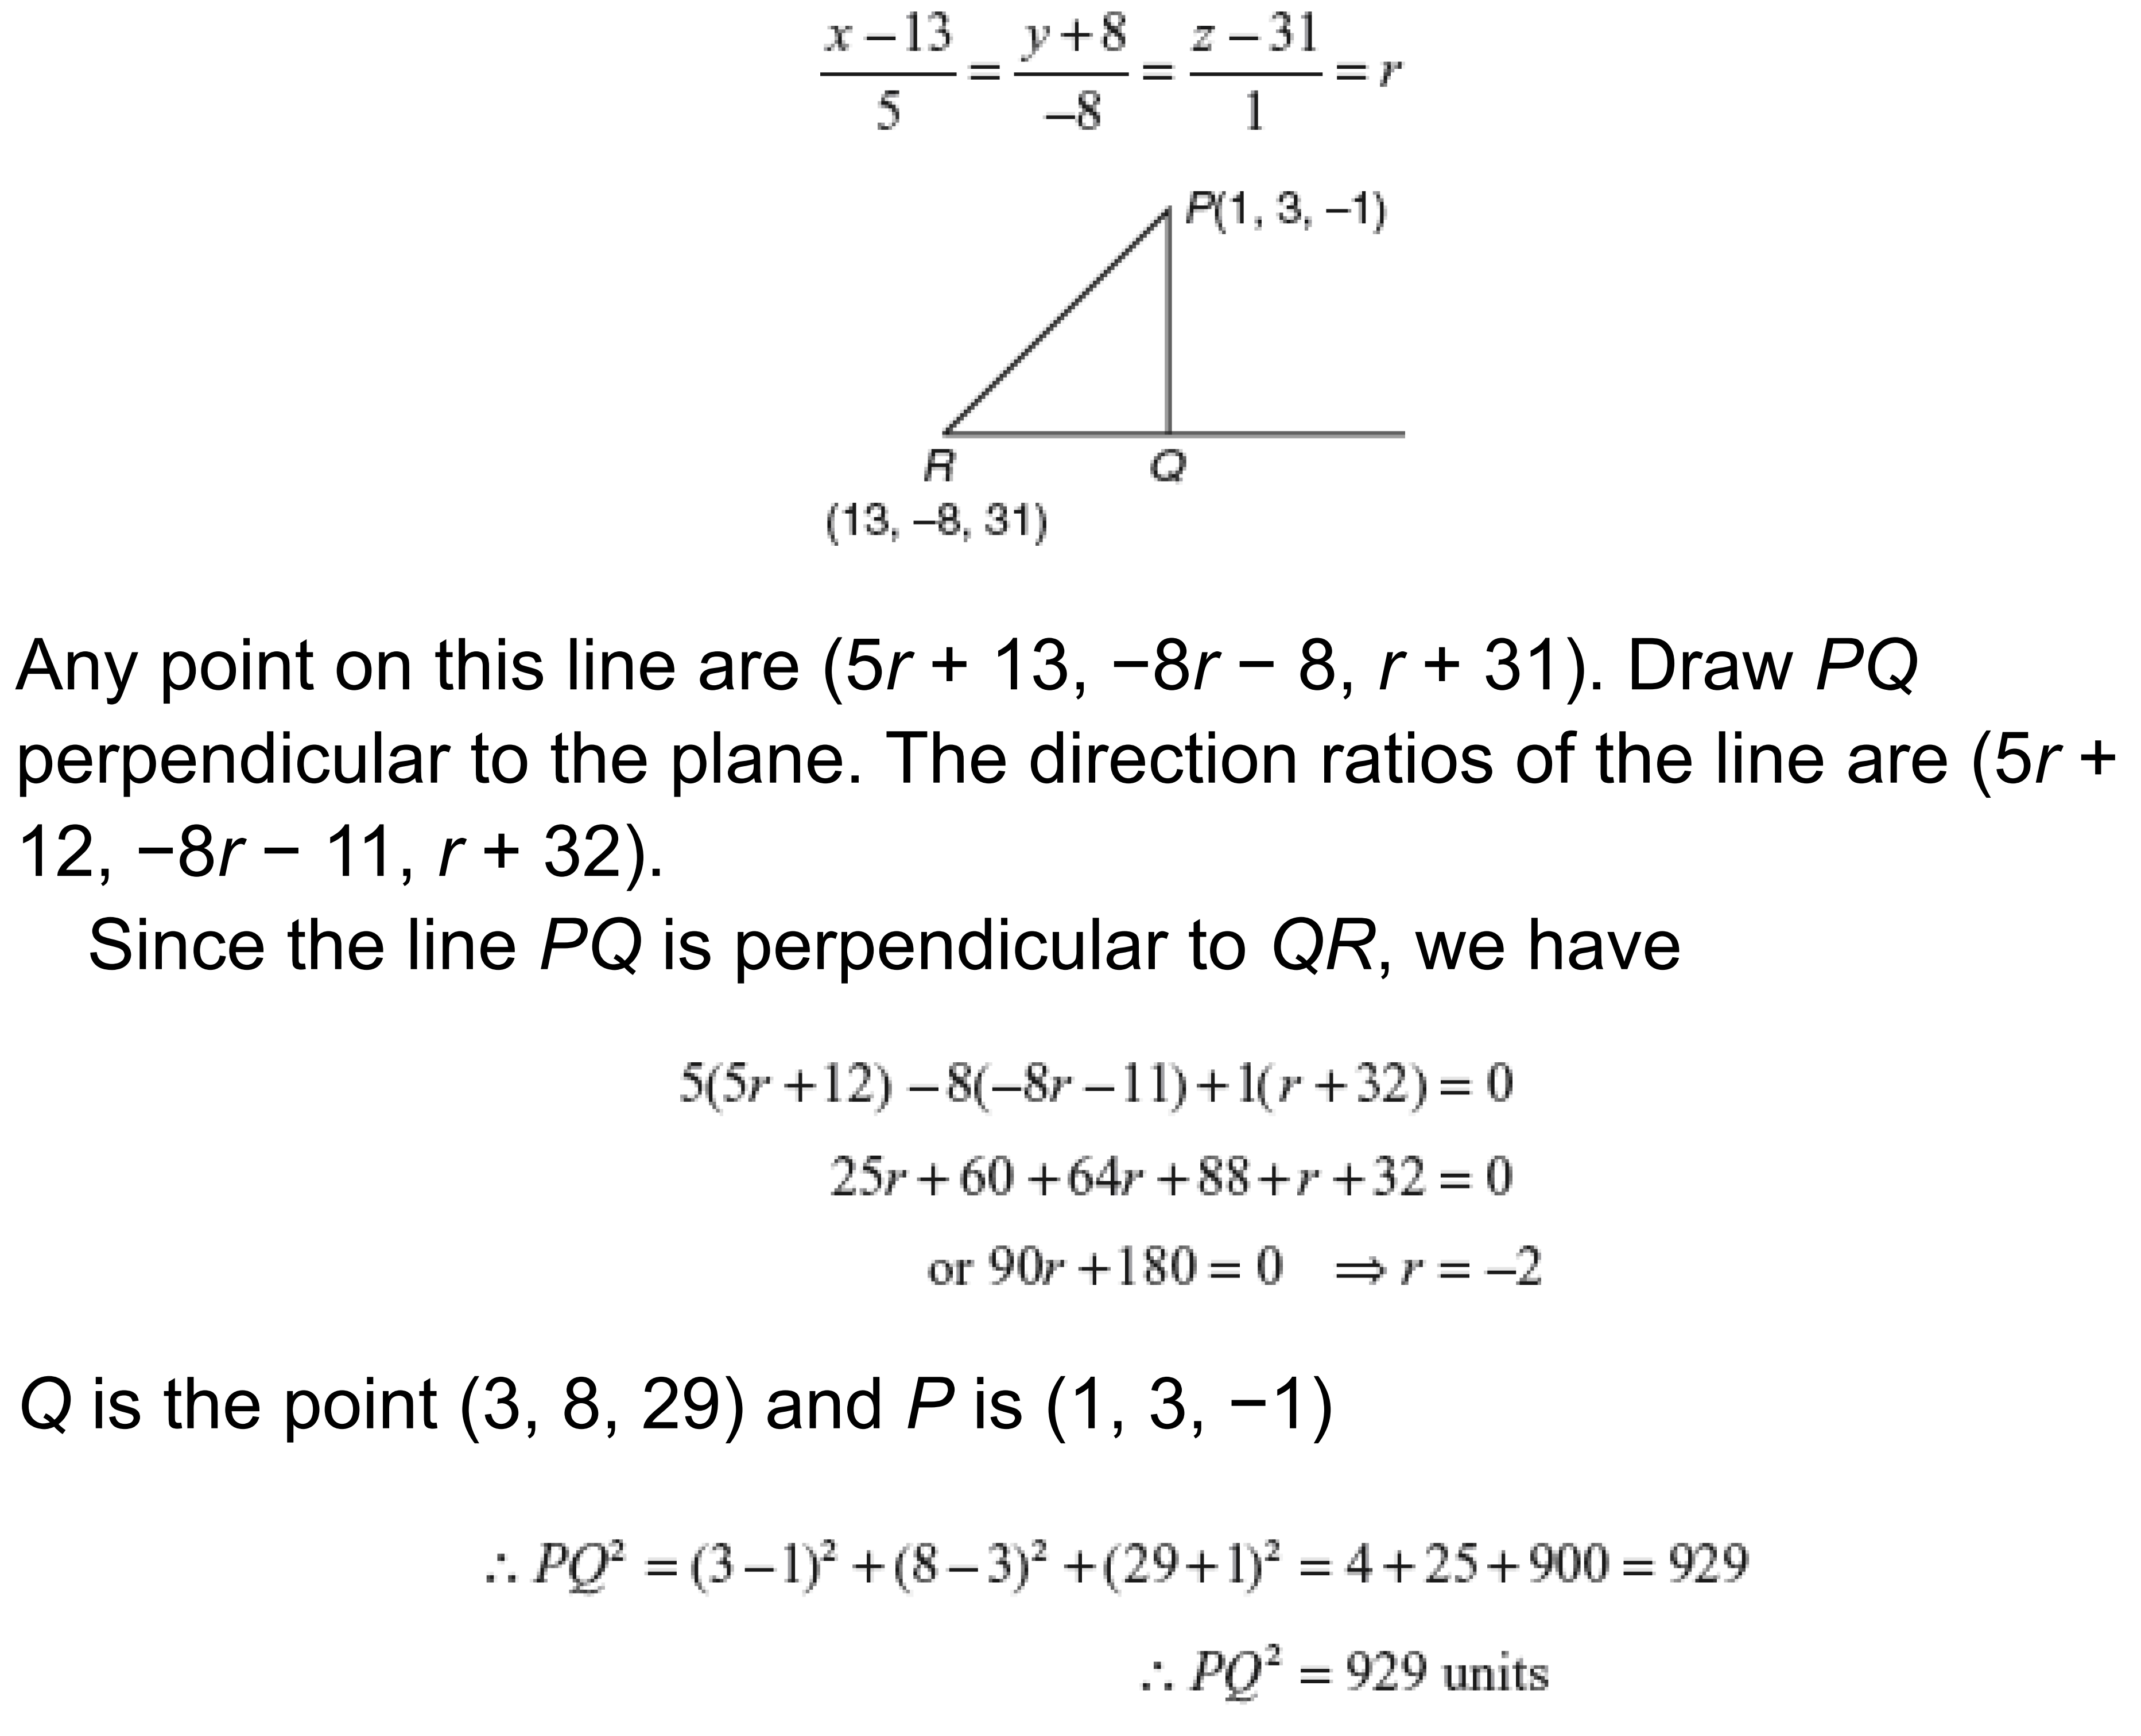
\includegraphics[height=5.5cm,width=1\textwidth,keepaspectratio]{4ans.png}
            % \caption{caption_name}
            \label{fig:4ans.png}
        \end{figure}
    }
\end{frame}

\begin{frame}[t]{Formulas of distances (Umnov 107)}
    \framesubtitle{Line to line}
    \begin{minipage}{0.6\textwidth}
        \textbf{\textit{Line to line}}\begin{itemize}
            \item \textit{if collinear} $d = \dfrac{|(\vec{r_2}-\vec{r_1}) \times \vec{a_1}| }{|\vec{a_1}|}$, where \\ $\vec{r_{1,2}}$ - are points of lines and $a_1$ -- directed vector of one line
            \item \textit{if skew} $d = \dfrac{|(\vec{r_2}-\vec{r_1},\vec{a_1},\vec{a_2})| }{|\vec{a_1}\times\vec{a_2}|}$, where \\ $\vec{r_{1,2}}$ - are points of lines and $a_1$ -- direction vector of one line
        \end{itemize}
    \end{minipage}
    \begin{minipage}{0.39\textwidth}
        \begin{figure}[H]
            \centering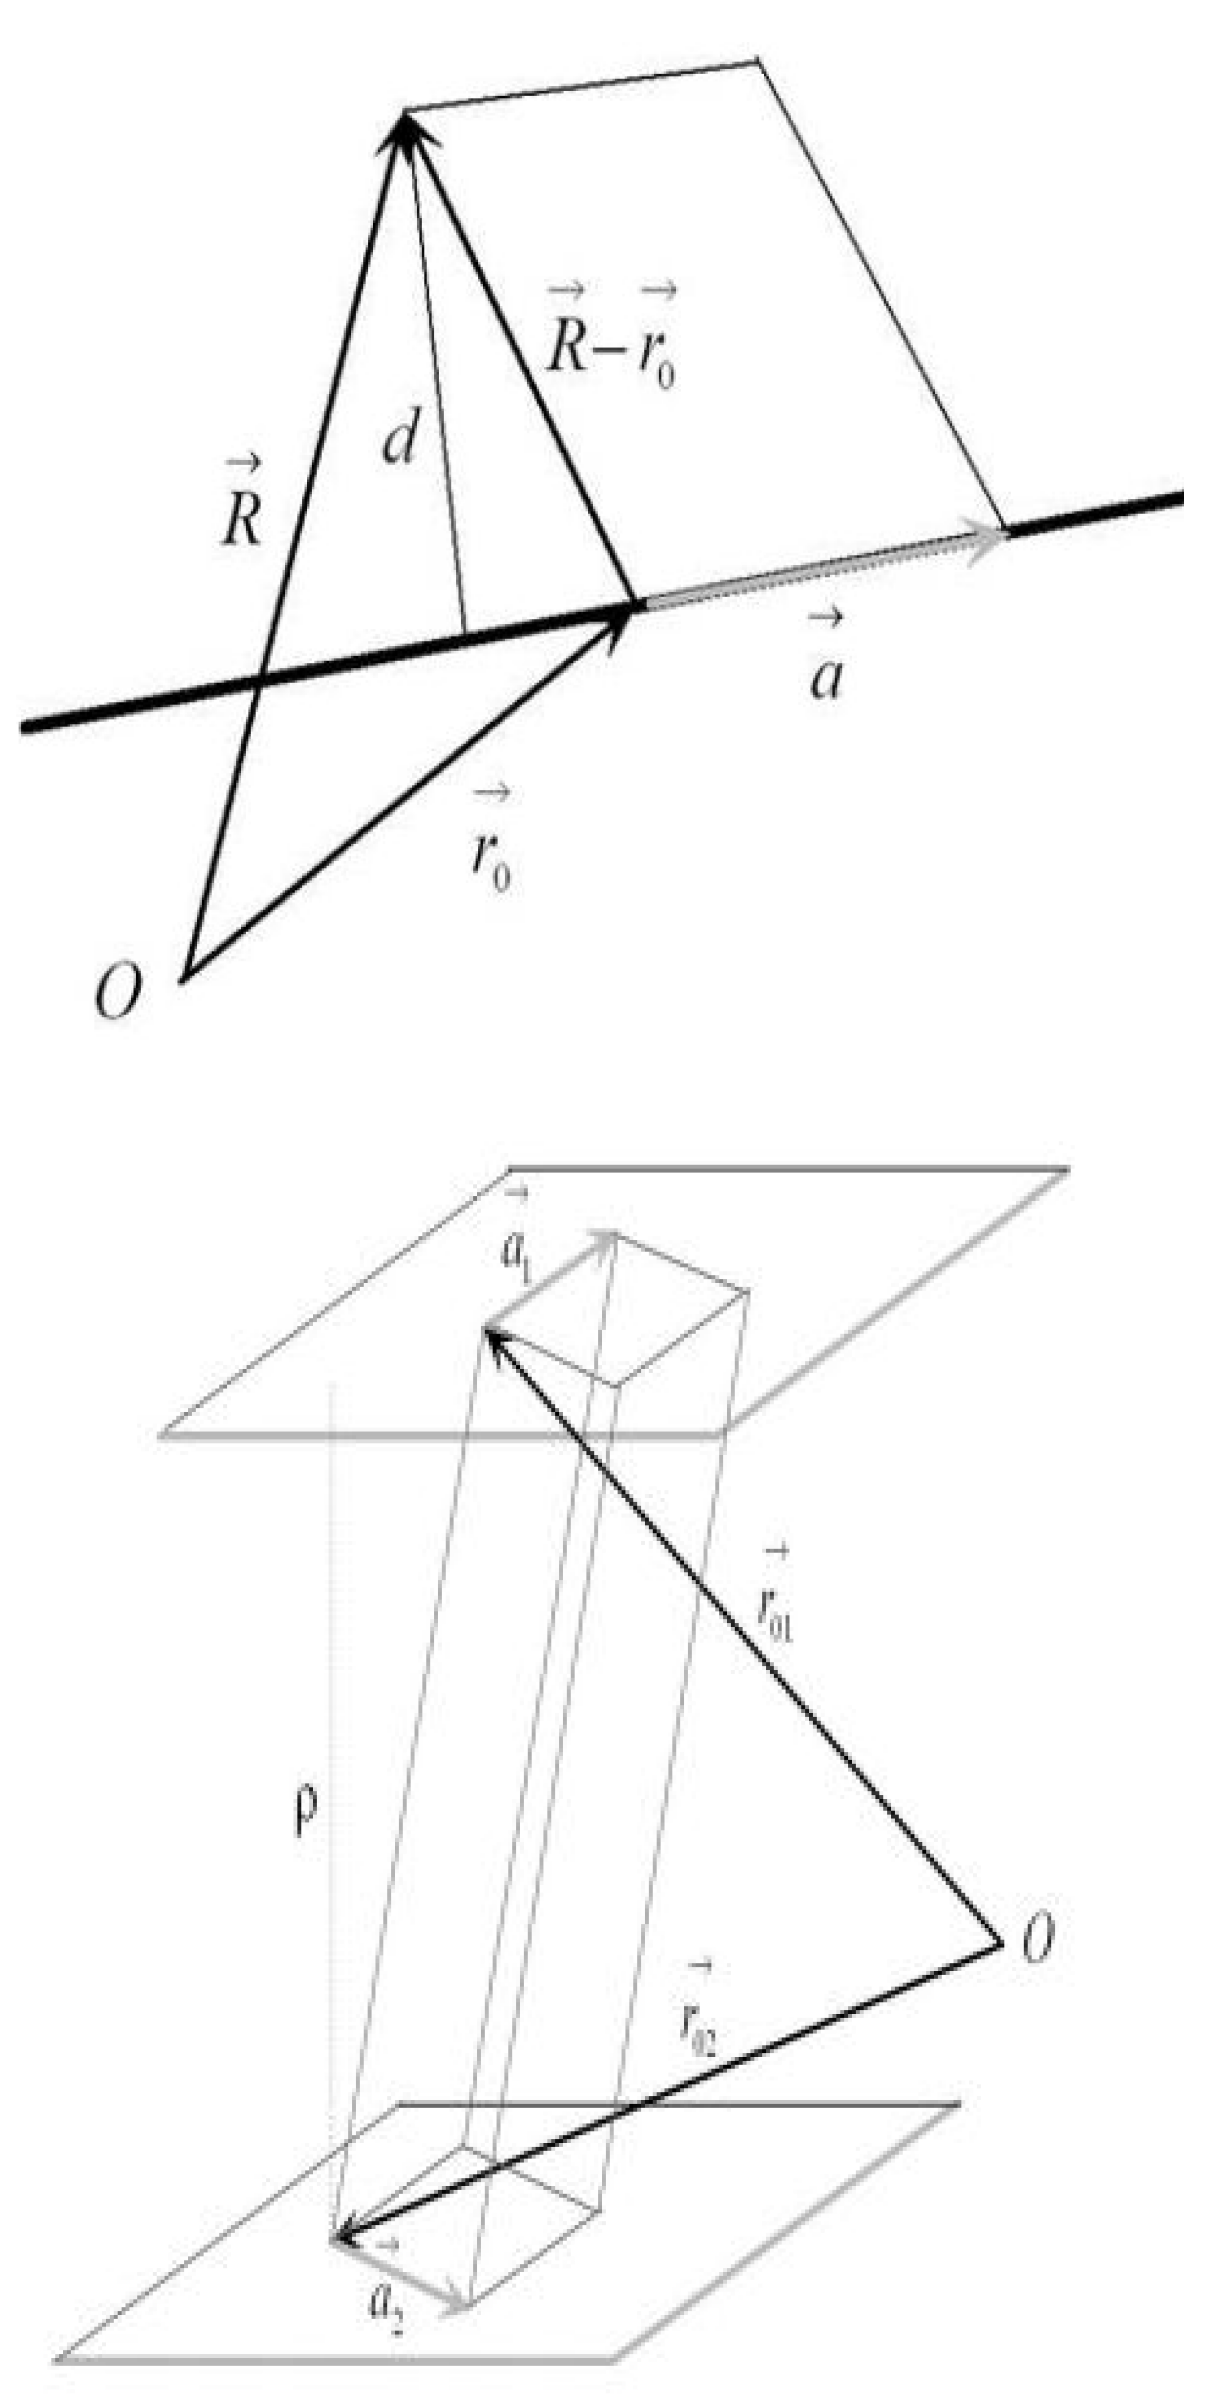
\includegraphics[height=5cm,width=1\textwidth,keepaspectratio]{distance_2.png}
            \label{fig:distance_2.png}
        \end{figure}
    \end{minipage}
\end{frame}

\begin{frame}[t]{Task 5}
    \framesubtitle{}
    \only<1>{
        \begin{minipage}{0.6\textwidth}
            Find the distance of the point $(1, -2, 3)$ from the plane $x - y + z = 5$ measured parallel to the line $\dfrac{x}{2} = \dfrac{y}{3} = \dfrac{z}{-6}$. And draw the picture.
        \end{minipage}
        \begin{minipage}{0.39\textwidth}
            \begin{figure}[H]
                \href{https://www.geogebra.org/3d/fvfbfwjc}{
                    \centering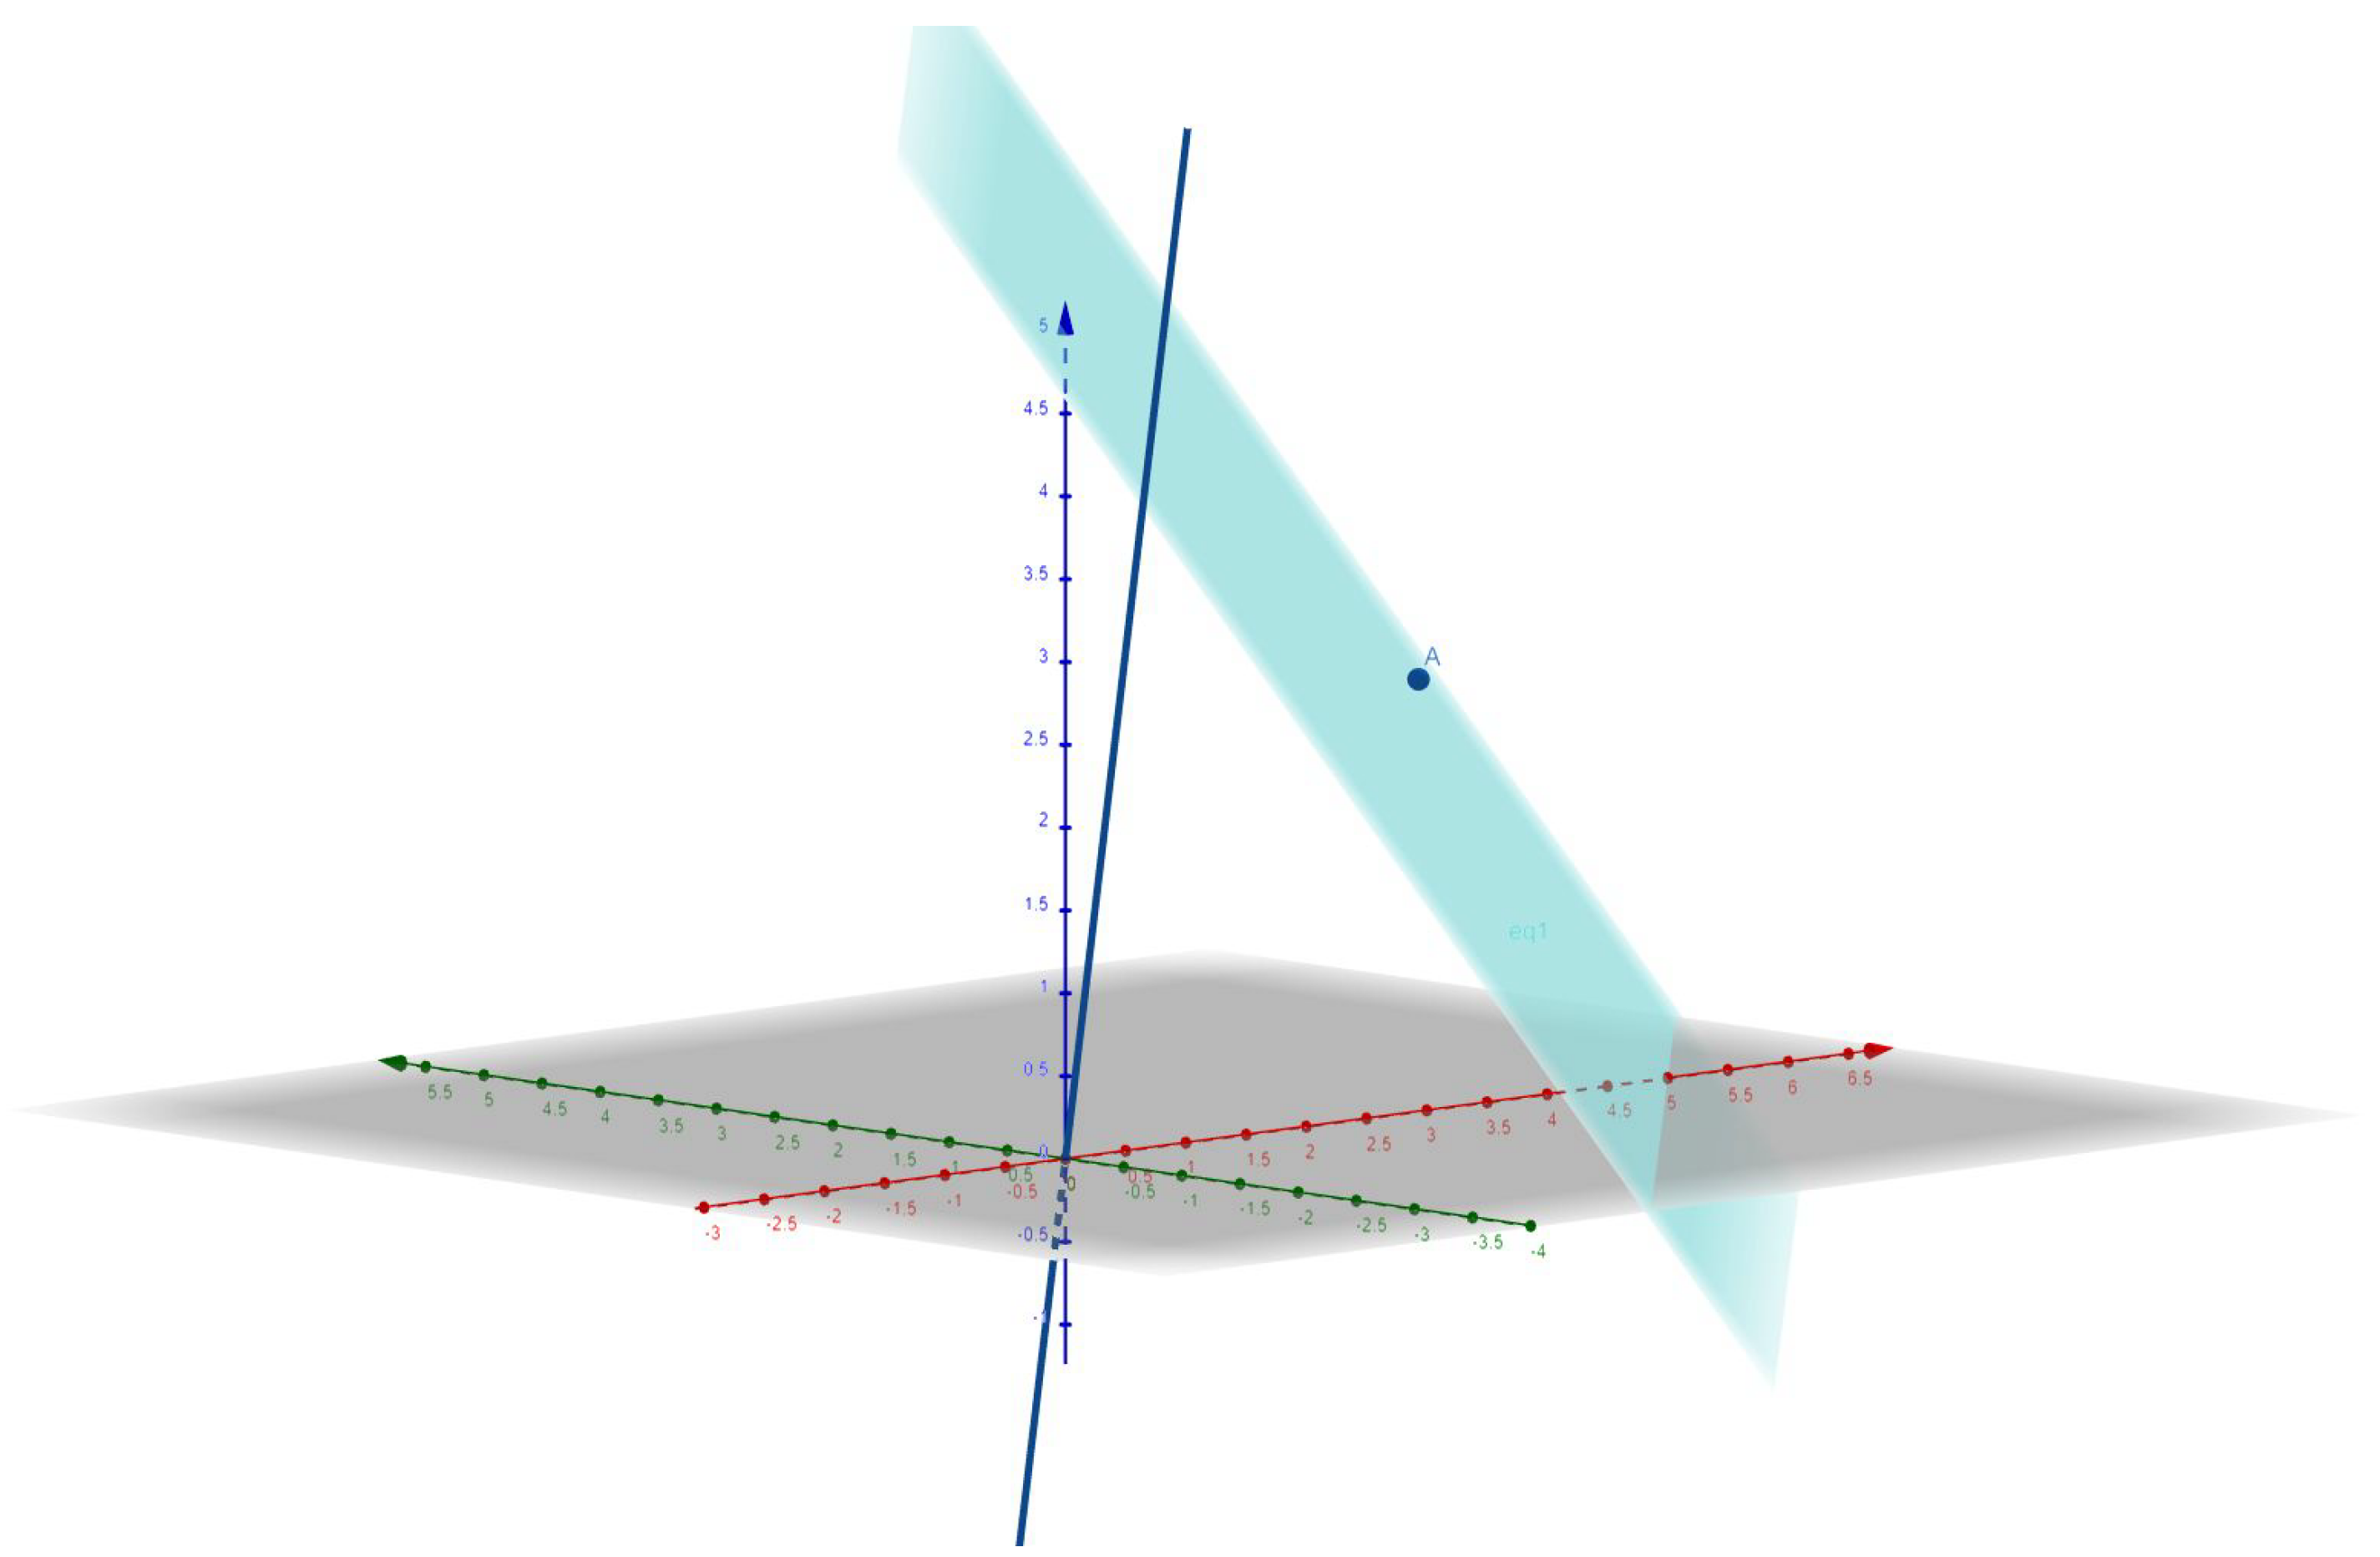
\includegraphics[height=6cm,width=1\textwidth,keepaspectratio]{5_fig.png}}
                % \caption{caption_name}
                \label{fig:5_fig.png}
            \end{figure}
        \end{minipage}}
    \only<2>{
        \alert{\Large Answer}
        \begin{figure}[H]
            \centering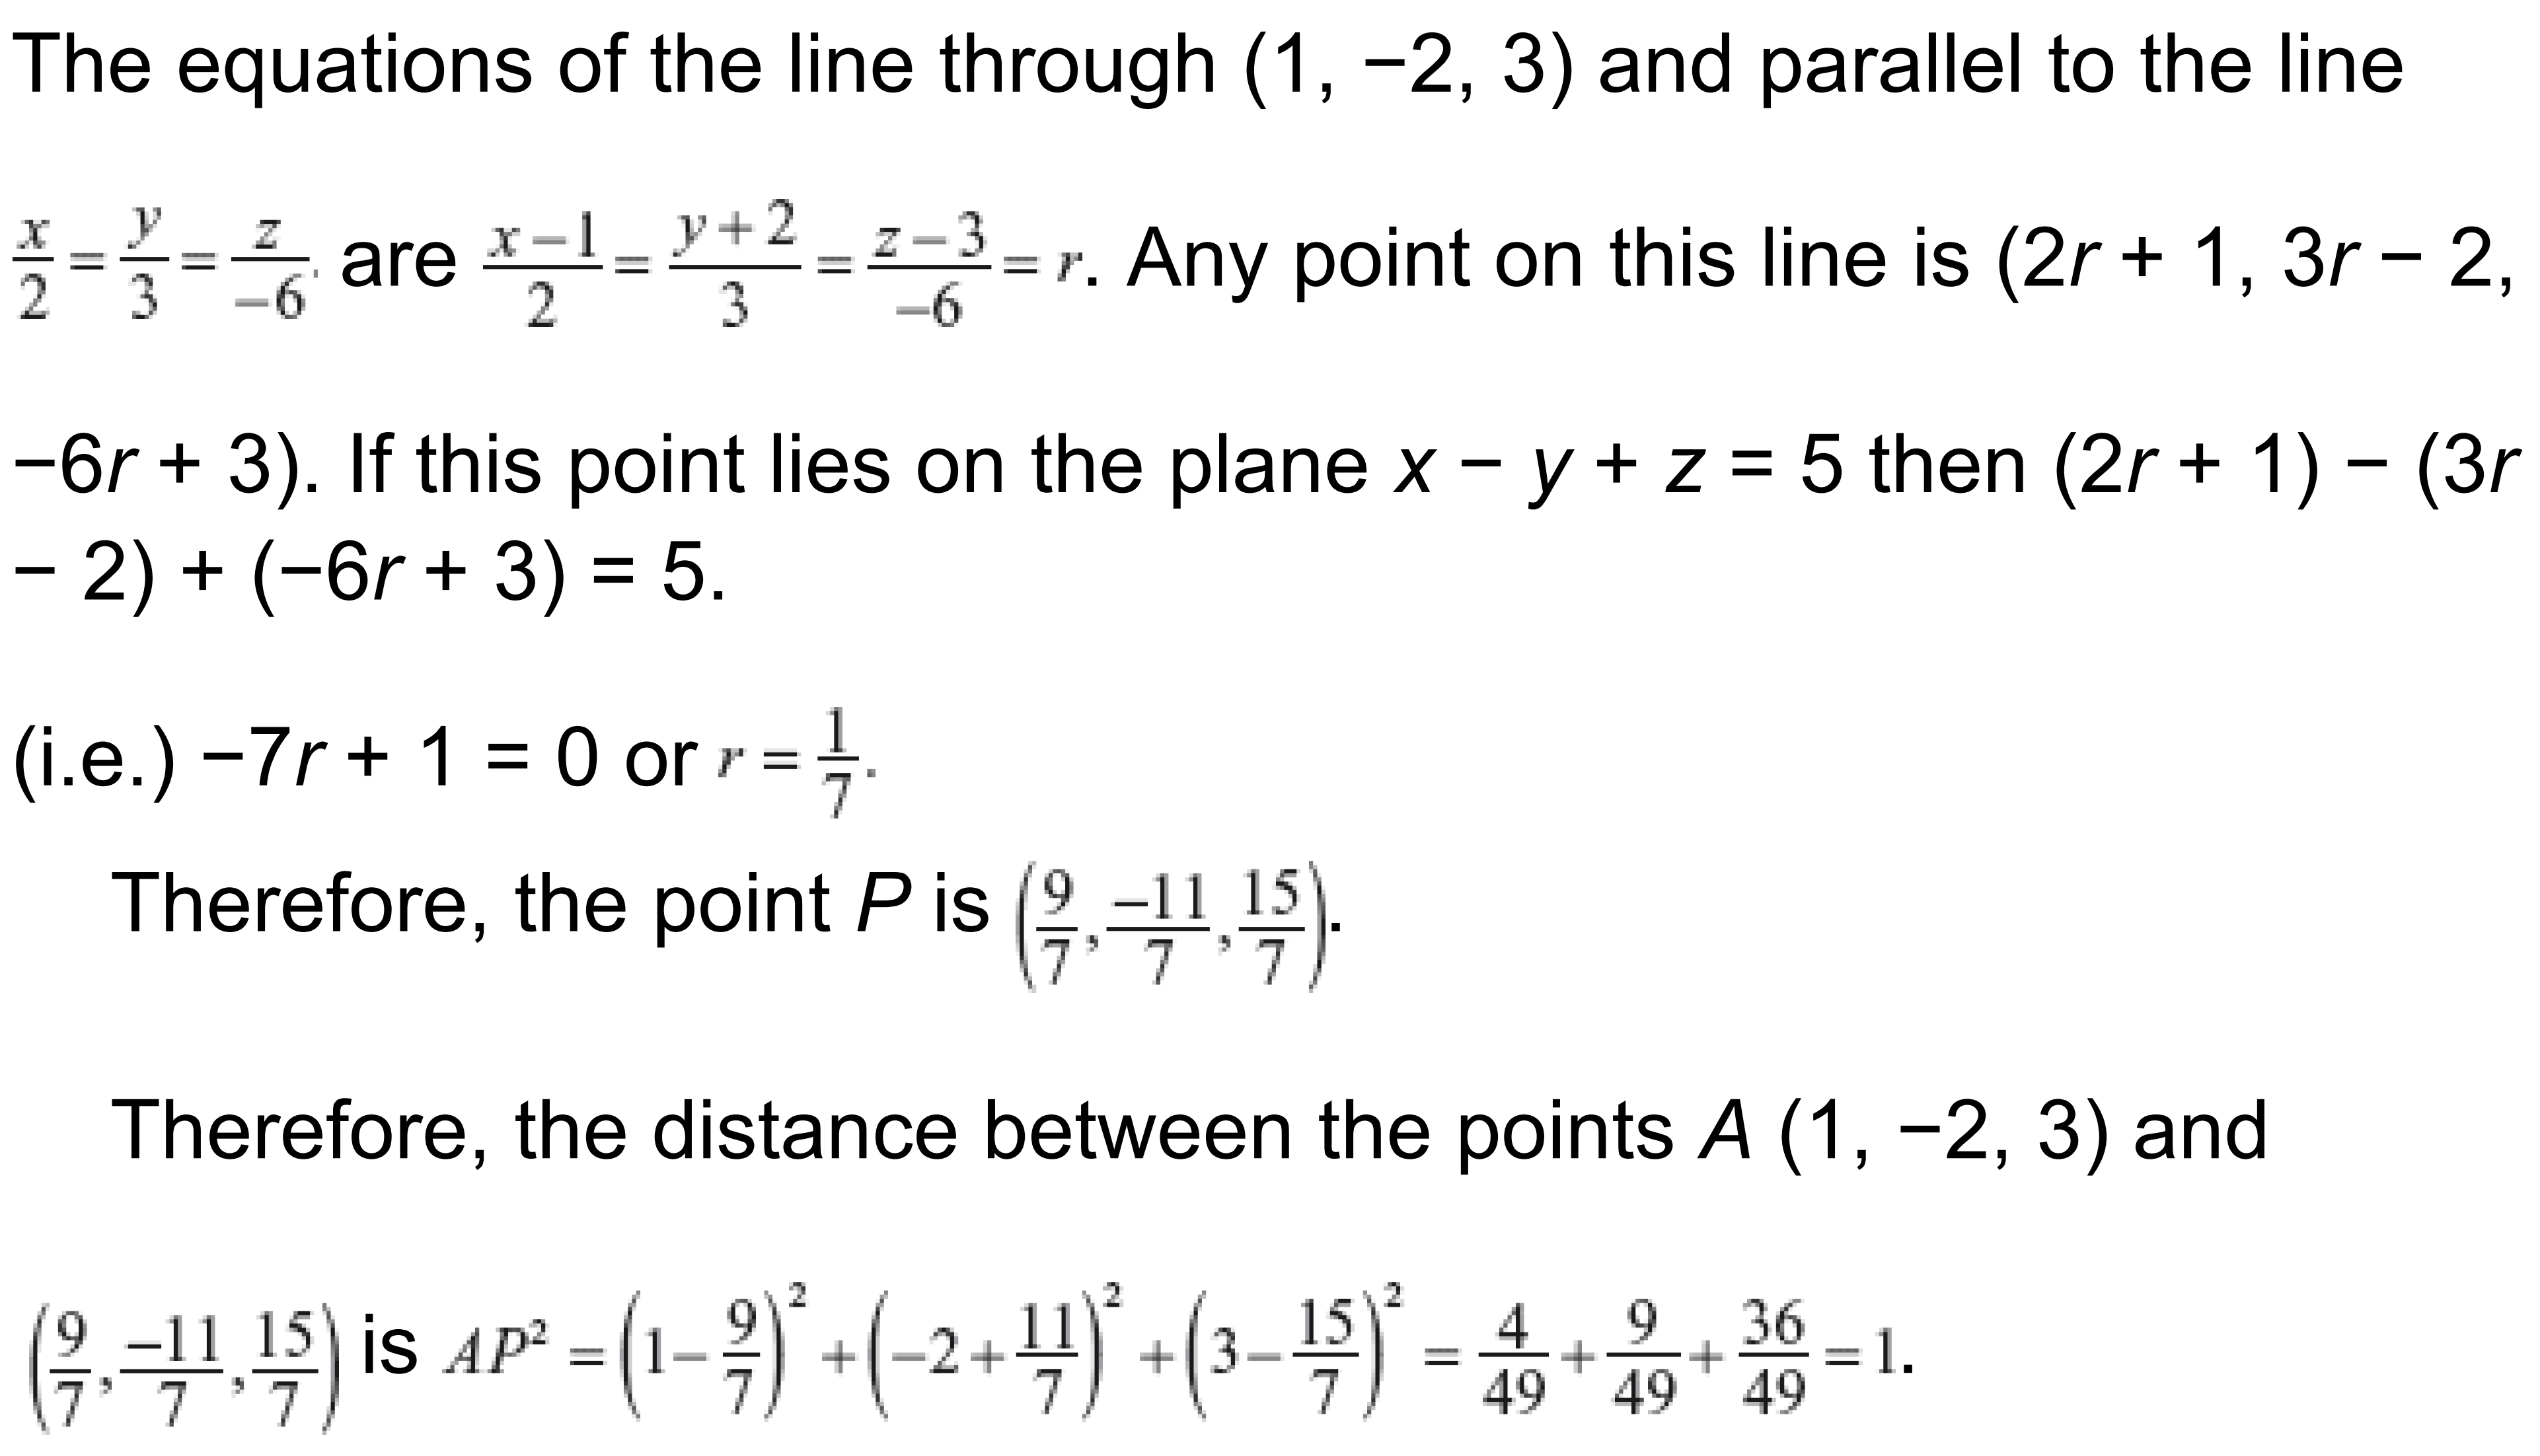
\includegraphics[height=5.5cm,width=1\textwidth,keepaspectratio]{5ans.png}
            % \caption{caption_name}
            \label{fig:5ans.png}
        \end{figure}
    }
\end{frame}

\begin{frame}[t]{Task 6}
    \framesubtitle{}
    \only<1>{
        \vspace{-0.35cm}
        Draw the following three cases and find how much solutions does the systems have.
        \begin{enumerate}
            \item
                  $
                      \begin{cases}
                          2x + 3y - z = 1, \\
                          x - 2y + z = 2,  \\
                          x + y + z = 1
                      \end{cases}
                  $

            \item
                  $
                      \begin{cases}
                          2x - 3y + z = 3, \\
                          x - 2y + 2z = 2, \\
                          x - y - z = 1
                      \end{cases}
                  $

            \item
                  $
                      \begin{cases}
                          2x - 3y + z = 3, \\
                          x - 2y + 2z = 0, \\
                          x - y - z = 1
                      \end{cases}
                  $

        \end{enumerate}}
    \only<2>{
        \alert{\Large Answer}
        \vspace{-0.3cm}
        \begin{figure}[H]
            \begin{subfigure}[t]{0.30\textwidth}
                \href{https://www.geogebra.org/calculator/axdfufzx}{\centering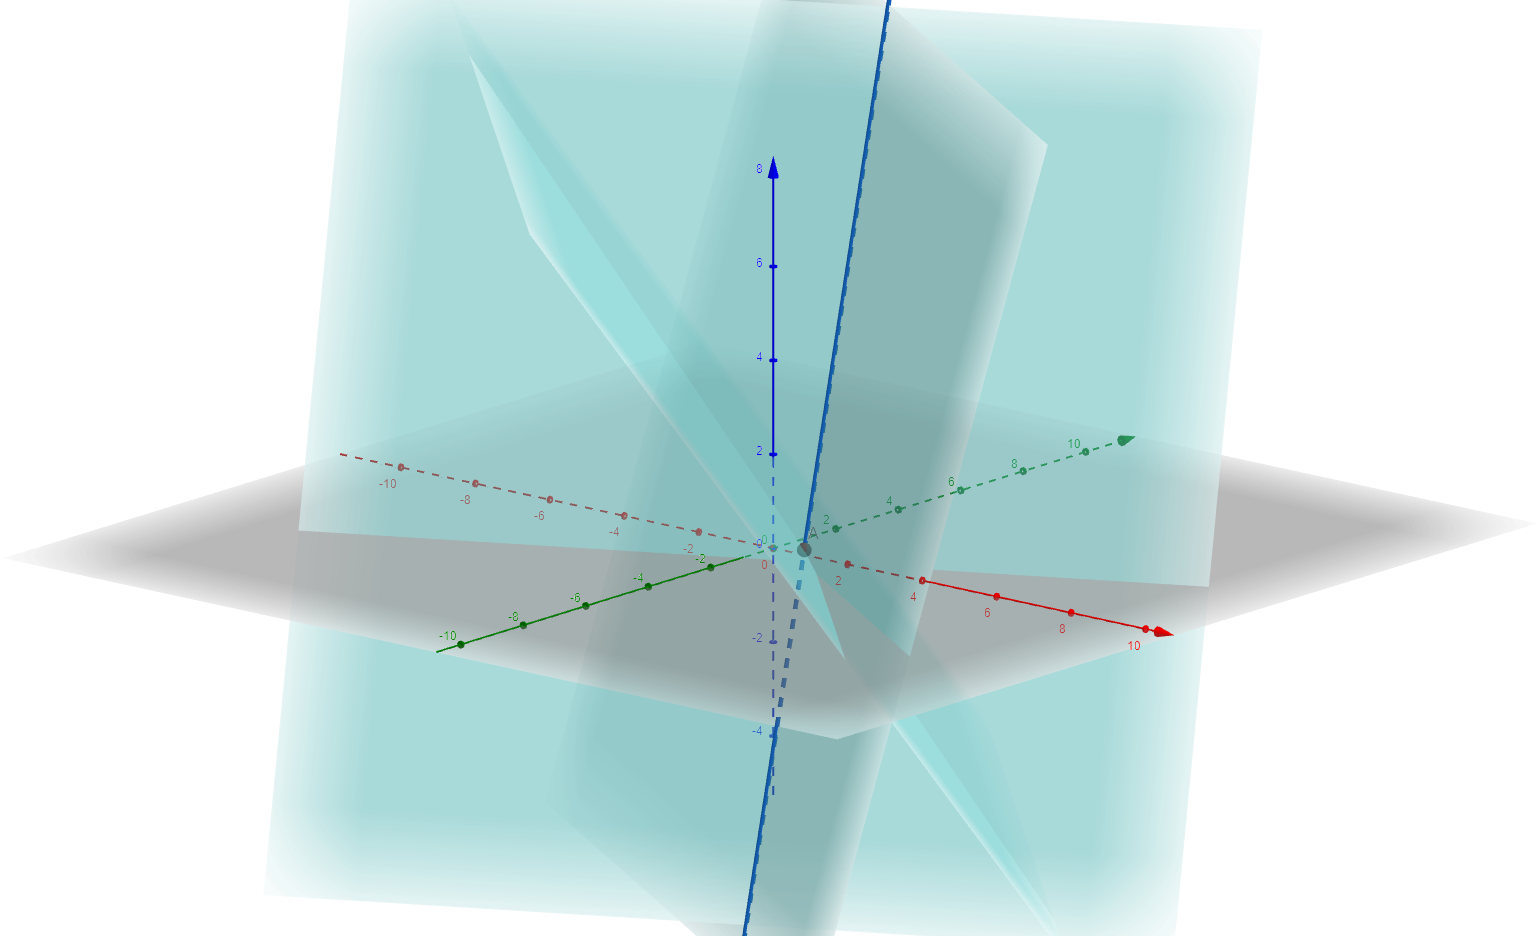
\includegraphics[height=6cm,width=1\textwidth,keepaspectratio]{lab7_task6_1.png}}
                \caption*{1. $\left[
                    \begin{array}{ccc|c}
                    1 & 0 & 0 & 10/9 \\
                    0 & 1 & 0 & -1/3 \\
                    0 & 0 & 1 & 2/9 \\
                    \end{array}
                    \right]$ \\ \textbf{Point}}
                \label{fig:lab7_task6_1.png}
            \end{subfigure}
            \begin{subfigure}[t]{0.30\textwidth}
                \href{https://www.geogebra.org/calculator/veshzb2c}{\centering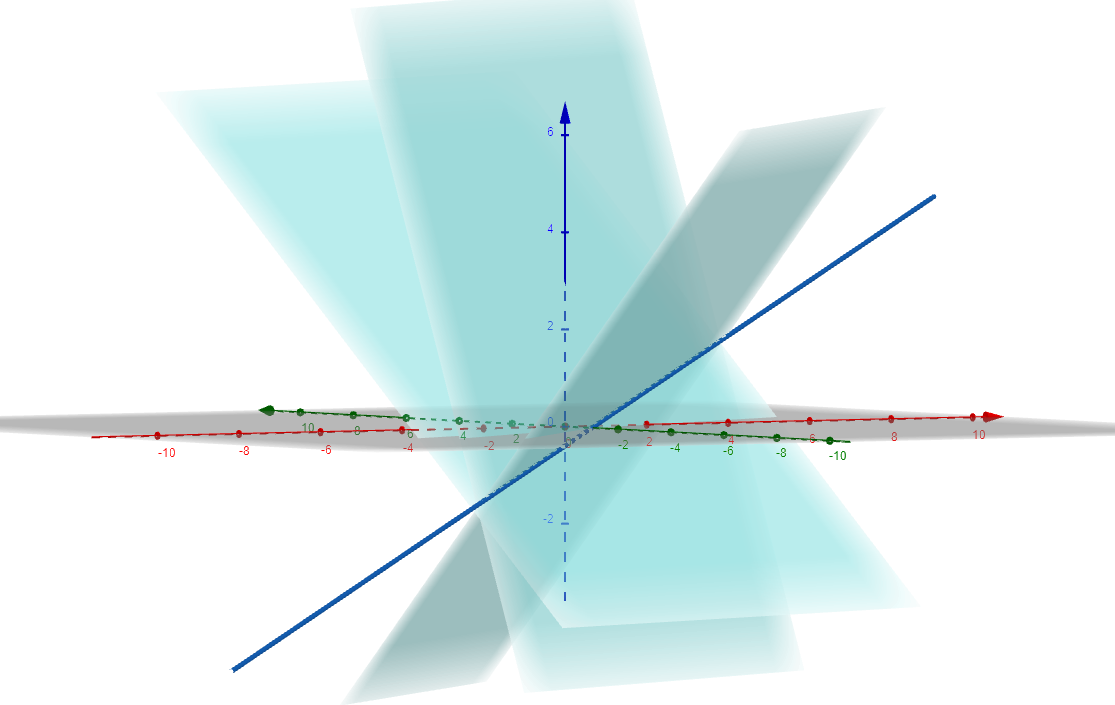
\includegraphics[height=6cm,width=1\textwidth,keepaspectratio]{lab7_task6_2.png}}
                \caption*{2. $\left[
                    \begin{array}{ccc|c}
                        1 & 0 & -4 & 0 \\
                        0 & 1 & -3 & -1 \\
                        0 & 0 & 0 & 0 \\
                        \end{array}
                    \right]$ \\ \textbf{Plane}}
                \label{fig:lab7_task6_2.png}
            \end{subfigure}
            \begin{subfigure}[t]{0.30\textwidth}
                \href{https://www.geogebra.org/calculator/zupzuscv}{\centering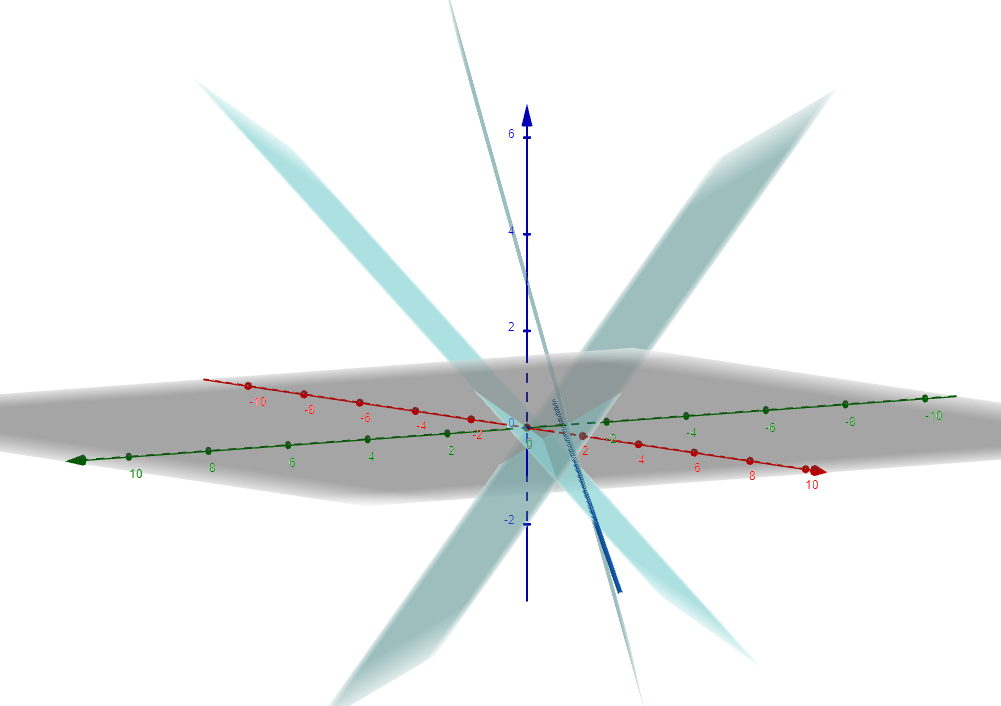
\includegraphics[height=6cm,width=1\textwidth,keepaspectratio]{lab7_task6_3.png}}
                \caption*{3. $\left[
                    \begin{array}{ccc|c}
                        1 & 0 & -4 & 6 \\
                        0 & 1 & -3 & 3 \\
                        0 & 0 & 0 & -2 \\
                        \end{array}
                    \right]$ \\ \textbf{No exists}}
                \label{fig:lab7_task6_3.png}
            \end{subfigure}
        \end{figure}
    }
\end{frame}

\begin{frame}[t]{Task 7}
    \framesubtitle{}
    \only<1>{
        Find the condition that one of the lines given by $ax^2 + 2hxy + by^2 = 0$ may be perpendicular to one of the lines given by $a_1x^2 + 2h_1xy + by^2 = 0$. And draw the picture.}
    \only<2>{
        \alert{\Large Answer}
        \begin{figure}[H]
            \centering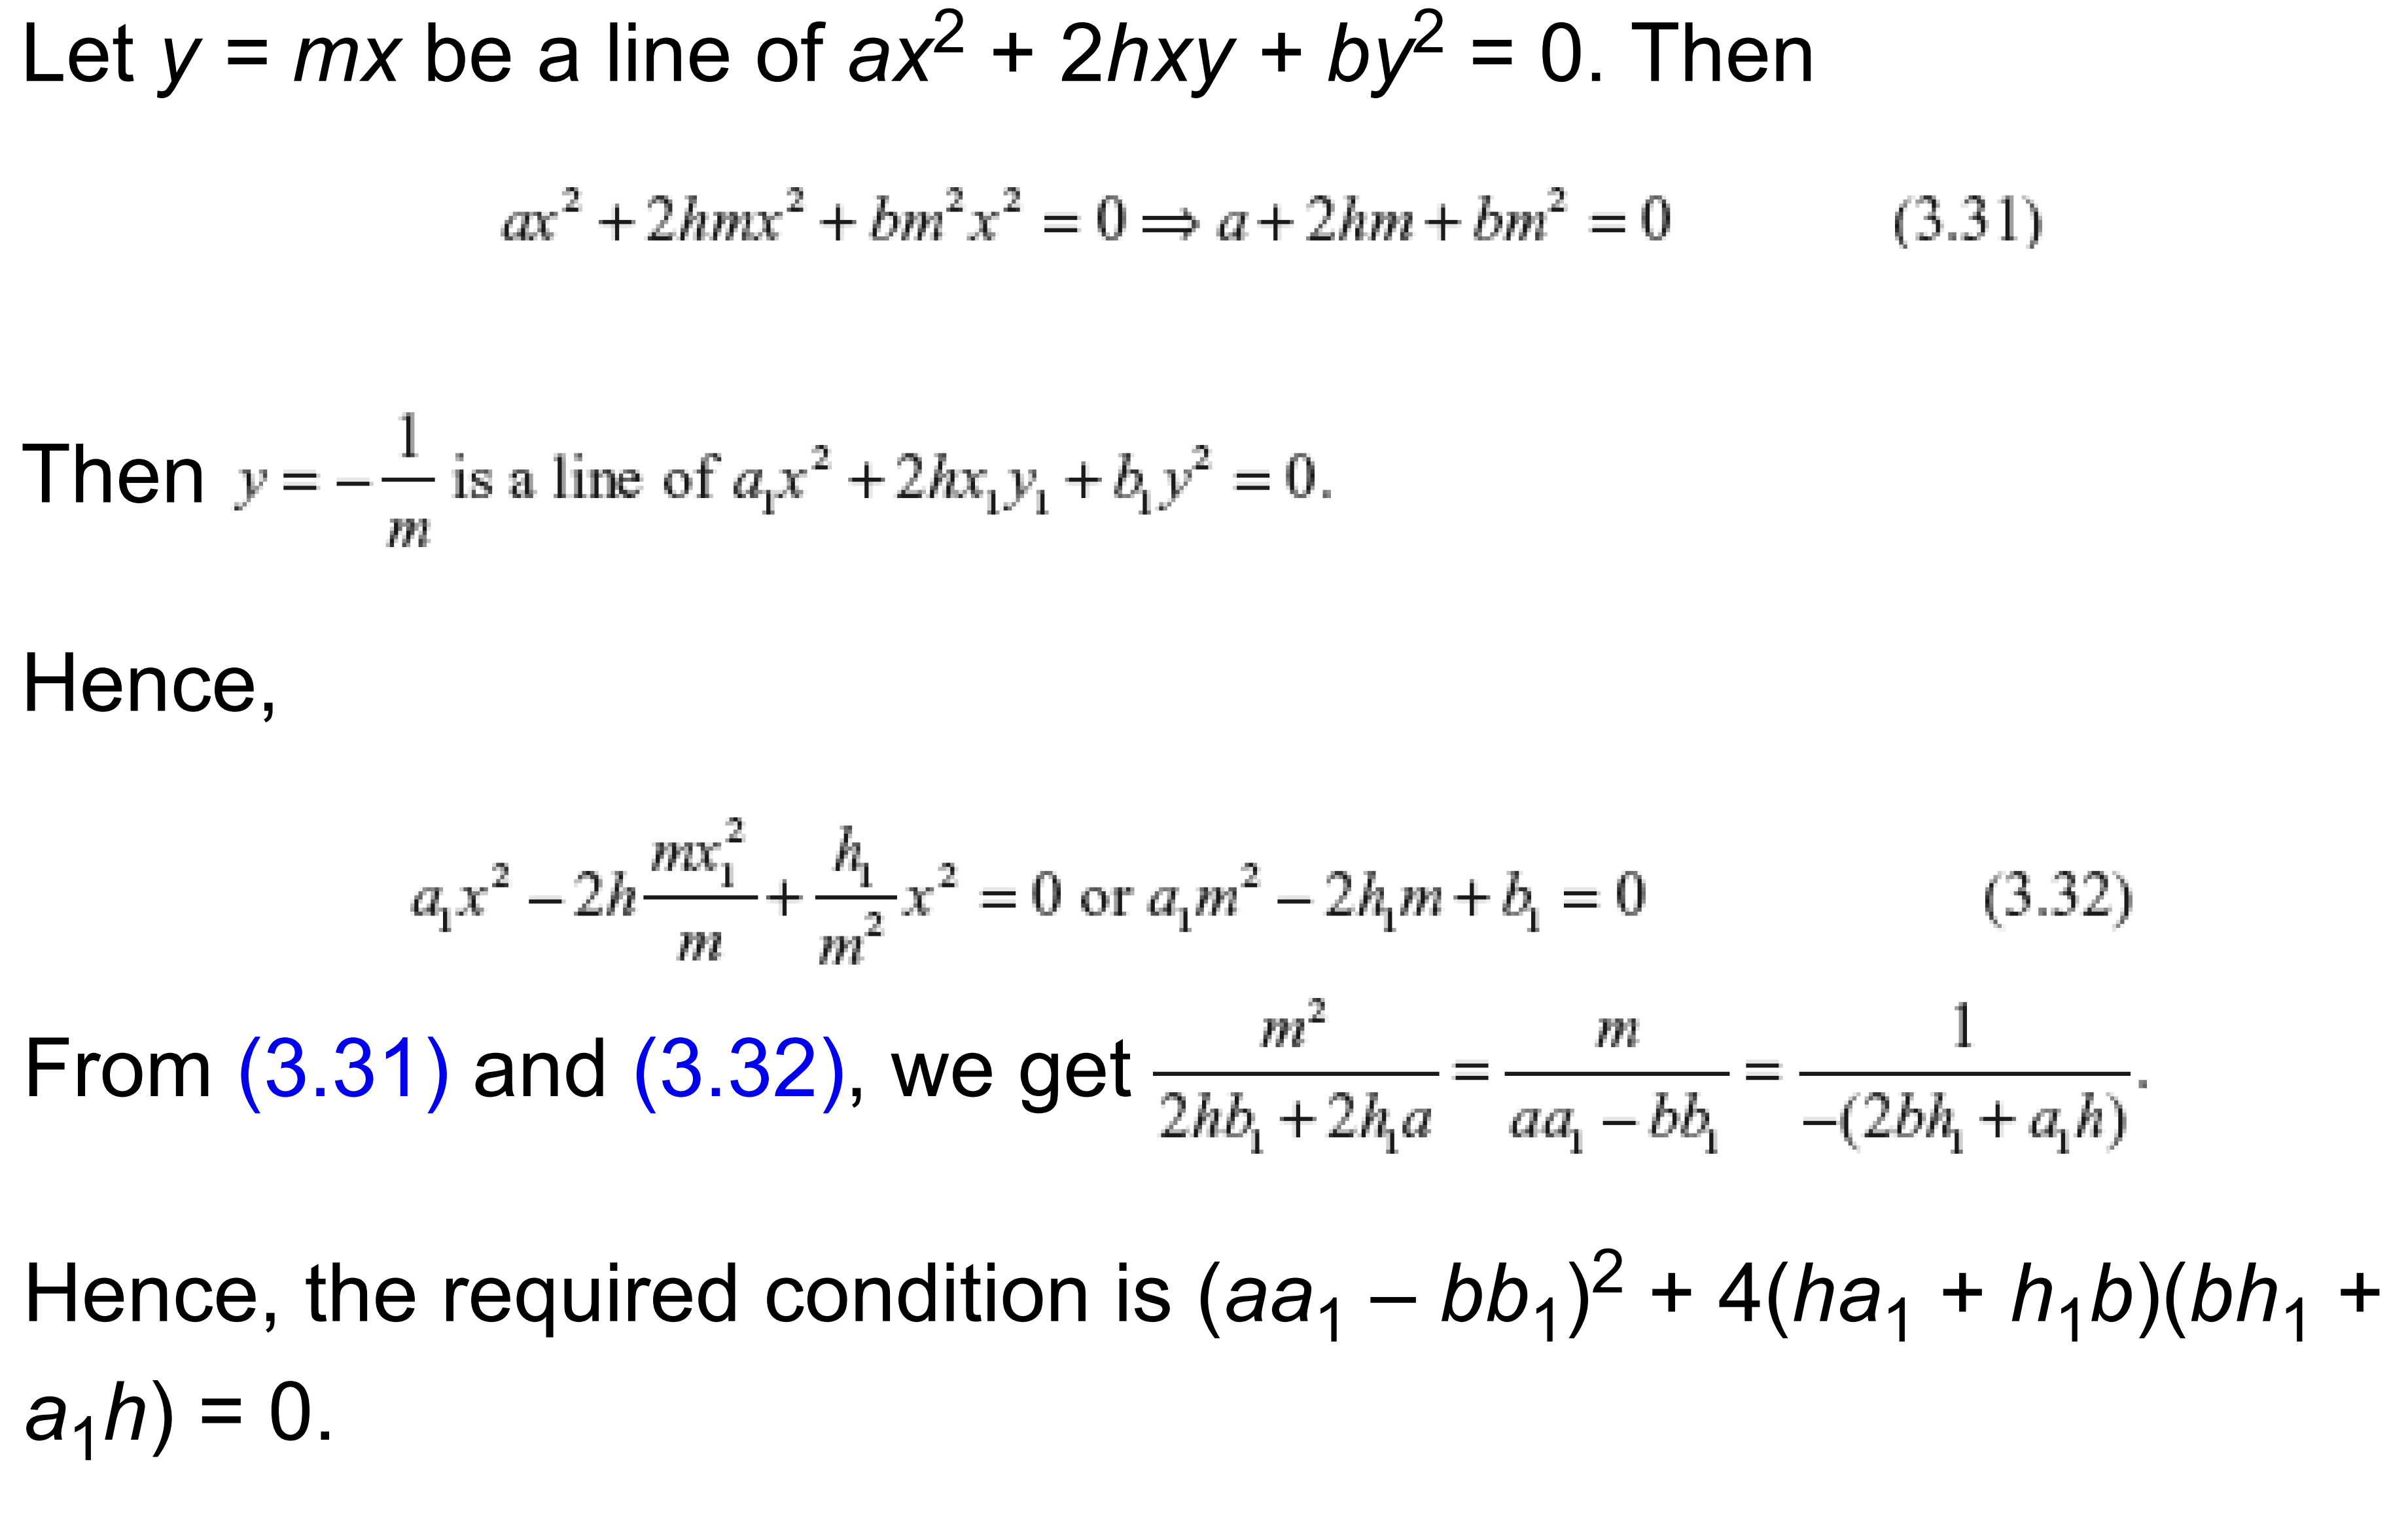
\includegraphics[height=5.5cm,width=1\textwidth,keepaspectratio]{7ans.png}
            % \caption{caption_name}
            \label{fig:7ans.png}
        \end{figure}
    }
\end{frame}

\begin{frame}[t]{Reference material}
    % \framesubtitle{OnlineMschool}
    \Large
    \begin{itemize}
        \item \href{https://onlinemschool.com/math/library/analytic_geometry/line/}{Line in space (OnlineMschool)}
        \item \href{https://onlinemschool.com/math/assistance/equation/gaus/}{Gauss elimination online (OnlineMSchool)}
    \end{itemize}
\end{frame}

\fbckg{fibeamer/figs/last_page.png}
\frame[plain]{}

\end{document}